\subsection{Fatos estilizados da economia norte-americana}\label{FatosEUA}

%Desse modo, a literatura do supermultiplicador é um contraponto ao \textit{trade-off} apontado por \textcite{solow_importance_1995} uma vez que são os gastos autônomos que lideram o crescimento no longo prazo.

%TODO Rever início da seção.

A participação do investimento das firmas na renda ---  e também nos trabalhos acadêmicos --- é bastante superior a do investimento das famílias. Tal pequenez (gráfico \ref{FigAutonomos}), no entanto, não implica em menor relevância para a dinâmica macroeconômica nem --- ao contrário do que indicaria a intuição --- em menor volatilidade (gráfico \ref{FigVolatilidade}). 
%TODO Pesquisar referência sobre subestimação da volatilidade do investimento residencial
Dito isso, pretende-se evidenciar que a importância deste gasto não se restringe a crise dos \textit{subprime} e não provém \textit{somente} das mudanças distributivas \cites{zezza_u.s._2008}{cardaci_inequality_2018} e do maior acesso ao crédito \cite{mian_consequences_2009}. 
Adicionalmente, procura-se mostrar que, ao contrário de \textcite{grebler_capital_1956}, tal relevância não só não se apequenou como tem se amplificado  \cites{fiebiger_semi-autonomous_2018}{karwowski_financialisation_2019}{walther_forty_2019}.
Em resumo, pretende-se mostrar que a pouca atenção dada ao investimento residencial não é compatível com seu grau de importância para a economia norte-americana e que esta relevância não se restringe à crise imobiliária recente.



%%%%%%%%%%%%%%%%%%%%%%%%%%%%% PEQUENA PARTICIPAÇÃO NO PIB %%%%%%%%%%%%%%%%%%%%%%%%%%%

\begin{figure}[H]
	\centering
	\caption{Participação dos gastos autônomos no PIB}
	\label{FigAutonomos}
	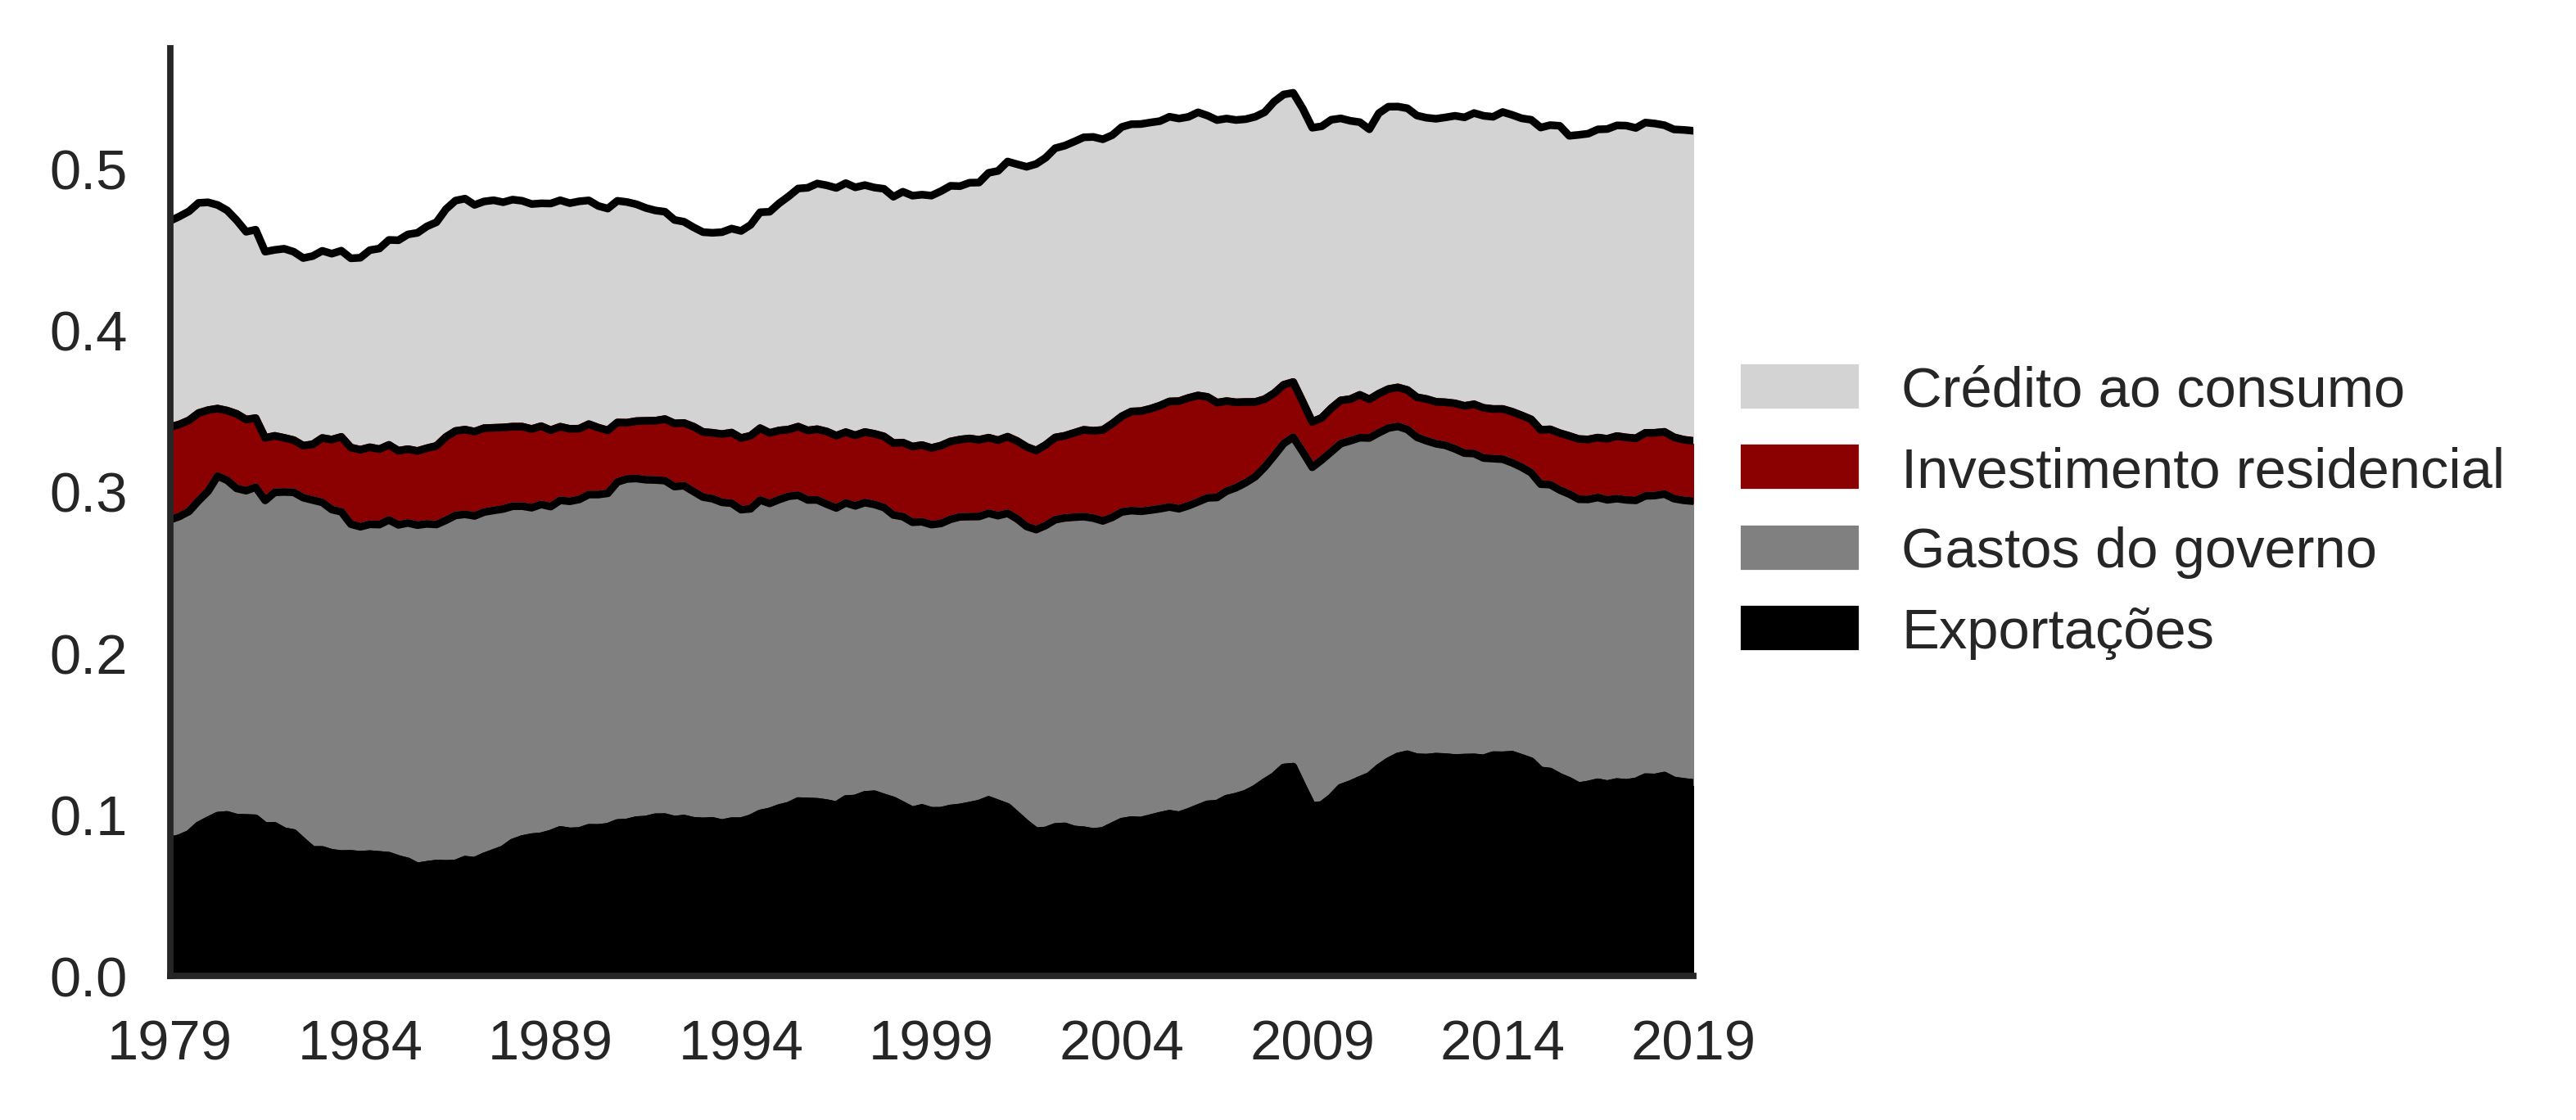
\includegraphics[width=\textwidth]{../../Dados/Fatos_Estilizados/figs/Gastos_autonomos.png}
	\caption*{\textbf{Fonte:} U.S. Bureau of Economic Analisys, elaboração própria}
\end{figure}


\begin{figure}[H]
	\centering
	\caption{Volatilidade de taxas de crescimento selecionadas (pré e pós-crise \textit{subprime})}
	\label{FigVolatilidade}
	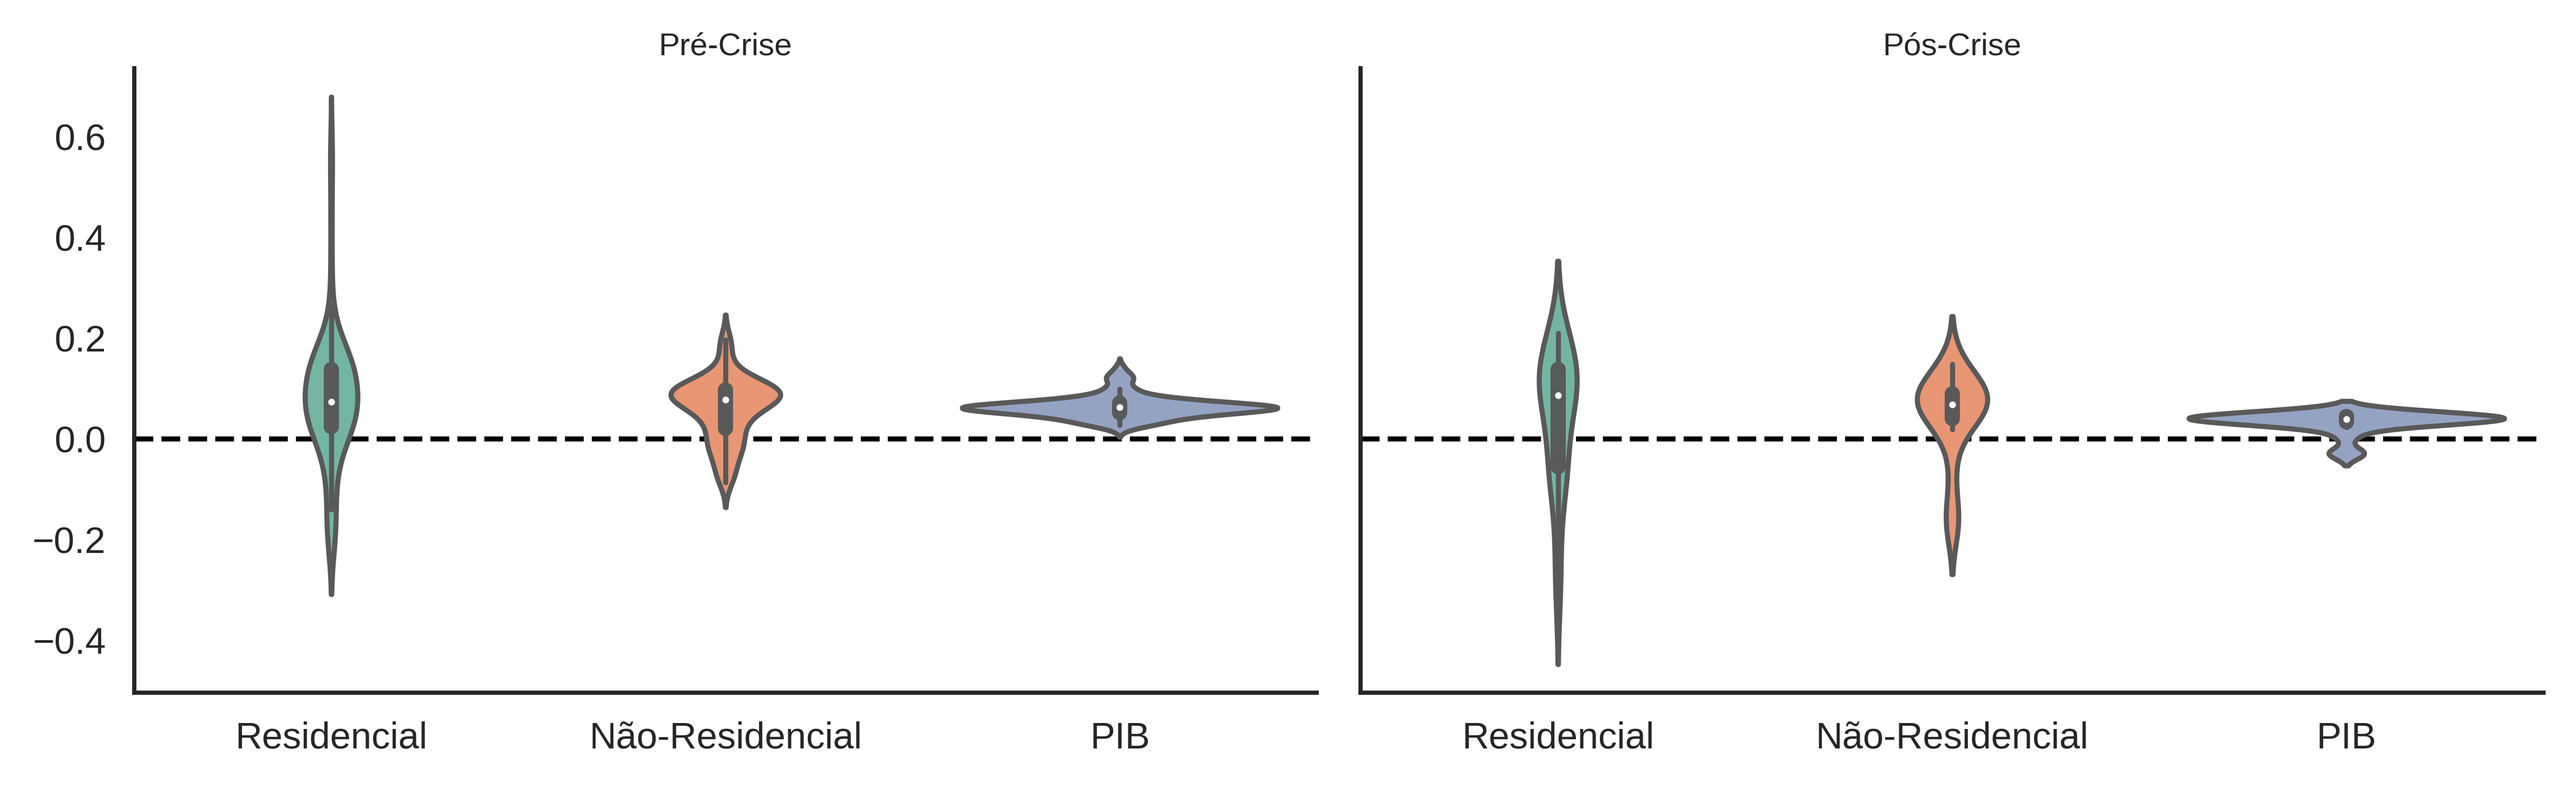
\includegraphics[width=\textwidth]{../../Dados/Fatos_Estilizados/figs/Volatilidade.png}
	\caption*{\textbf{Fonte:} U.S. Bureau of Economic Analisys, elaboração própria}
\end{figure}

Neste ponto, cabe mencionar o ineditismo de \textcite{green_follow_1997} e \textcite{leamer_housing_2007} --- e revisitado em \textcite{leamer_housing_2015} e por \textcite{fiebiger_trend_2017} --- ao lançar luz sobre a importância do investimento residencial na determinação dos ciclos econômicos antes mesmo da crise dos \textit{subprimes}. 
Ao avaliar o caso norte-americano, \textcite{green_follow_1997} conclui que o investimento residencial possui uma capacidade preditiva maior que o investimento das firmas, mas que isso não implica no estabelecimento de uma relação causal. Na tentativa de compreender tais resultados, afirma:

\begin{citacao}
	
	[P]erhaps residential investiment, like stock prices and interest rates, is a good predictor of GDP because it is a series that reflects \textbf{foward looking behavior}. Presumably households will not increase their expenditures on housing unless they expect to prosper in the future. Building a house is a natural mechanism for doing this. Thus, the series can do a good job of predicting GDP without necessarily causing GDP.
	\cite[p.~267, grifos adicionados]{green_follow_1997}
\end{citacao}
Apesar de dar atenção para um gasto não criador de capacidade, o argumento de \textcite{green_follow_1997} se difere das conclusões do supermultiplicador uma vez que não são estes gastos que lideram o crescimento.
\textcite{leamer_housing_2007}, por sua vez, avança em direção a relação de causalidade entre este gasto e o PIB. Grosso modo, afirma que a construção de novos imóveis implica em maior consumo de bens duráveis e, portanto, trata-se de um ciclo decorrente do \textit{volume} e não do preço dos imóveis. 

Uma forma de visualizar a importância do investimento residencial para o ciclo econômico na economia estadunidense é por meio do gráfico \ref{Investo_Resid} em que cada um dos painéis apresenta um ciclo iniciado no primeiro trimestre de crescimento positivo após a recessão\footnote{
	Raciocínio semelhante pode ser encontrado em \textcite{fiebiger_semi-autonomous_2018} em que, diferentemente do presente trabalho, não é incluído consumo financiado por crédito.}. 
No eixo vertical, observa-se a participação desse gasto no PIB, enquanto no eixo horizontal, o grau de utilização da capacidade como uma \textit{proxy} para o ciclo econômico. Exceto para o período 1991-2001, a recuperação (aumento da utilização da capacidade) é caracterizada por uma taxa de crescimento do investimento residencial maior que o crescimento da economia, resultando em maior participação desse gasto no PIB. Considerando que as firmas seguem o princípio do ajuste do estoque de capital, ampliam a taxa de acumulação de modo a ajustar o grau de utilização para o grau normal. O aumento da taxa de crescimento do investimento das firmas e de outros gastos reduz a participação do investimento residencial no PIB. A maturação do investimento das firmas, por sua vez, redunda em menor utilização da capacidade produtiva\footnote{
	Complementarmente, os trabalhos de \textcite{fiebiger_semi-autonomous_2018} e \textcite{fiebiger_trend_2017} também reportam o investimento residencial como determinante do comportamento cíclico e adicionam o consumo financiado por crédito a essa dinâmica. Além disso, apresentam uma similaridade com \textcite{dejuan_hidden_2017} e \textcite{teixeira_crescimento_2015} para os quais a instabilidade econômica está associada à instabilidade (ao menos de alguns) gastos autônomos e não do investimento das firmas, que segue o princípio do ajuste do estoque de capital.}. 



\begin{figure}[H]
	\centering
	\caption{Relação entre taxa de investimento residencial e grau de utilização por recessão}
	\label{FigIh_u}
	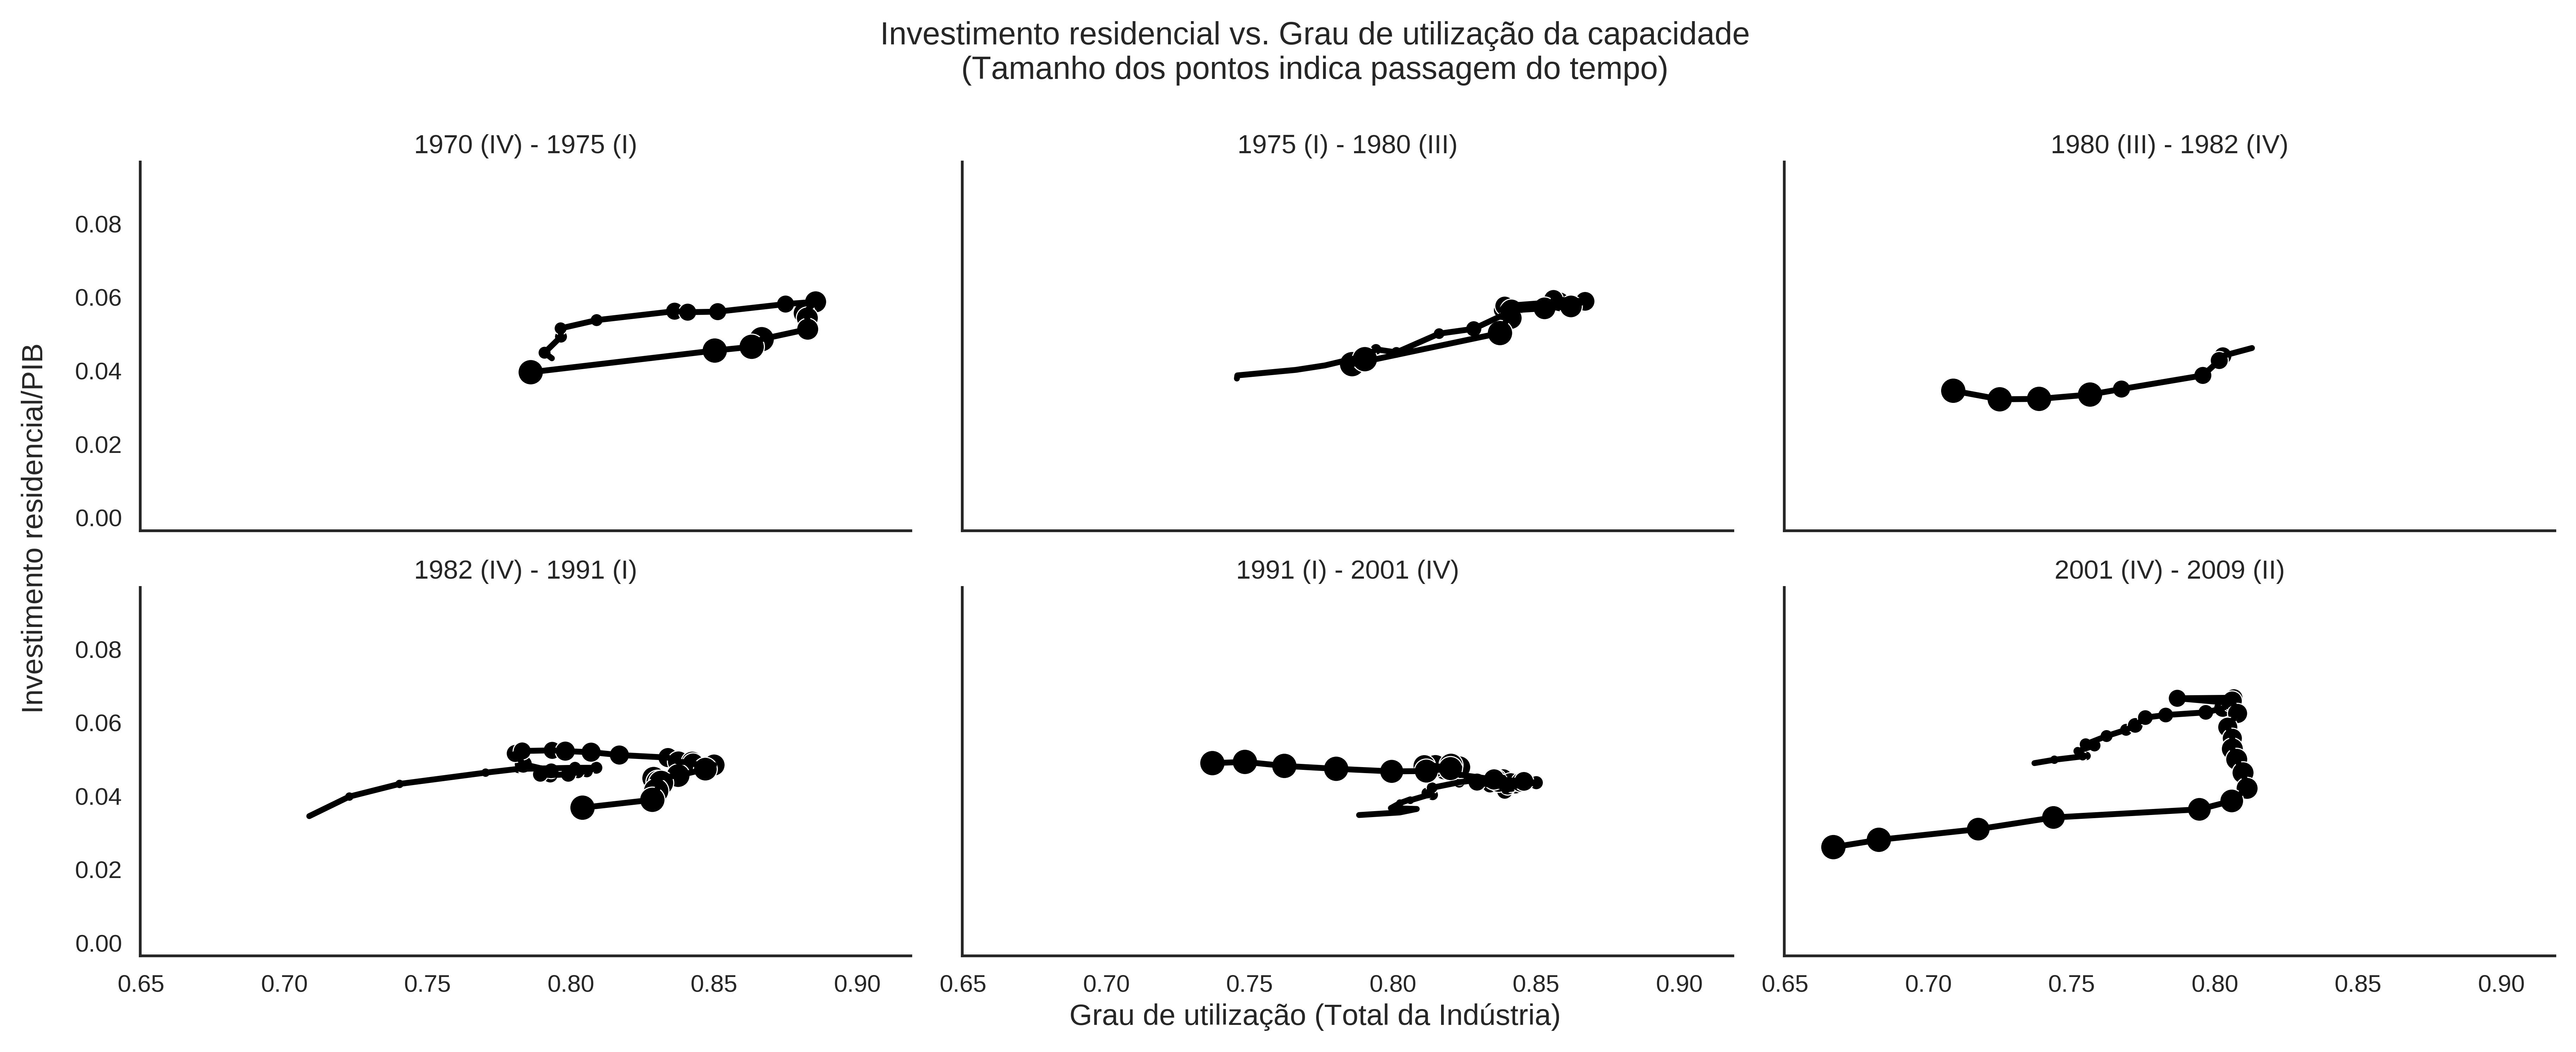
\includegraphics[width=\textwidth]{../../Dados/Fatos_Estilizados/figs/Ciclo_Ih_u.png}
	\caption*{\textbf{Fonte:} Elaboração própria}
\end{figure}

%%%%%%%%%%%%%%%%%%%%%%% GRÁFICO RELÓGIO DURÁVEIS %%%%%%%%%%%%%%%%%%

Uma forma de complementar tal discussão é por meio do gráfico \ref{FigInvesto_Duraveis} em que é feita a mesma periodização das crises dos painéis anterior com a diferença de que o eixo horizontal apresenta a participação do consumo de bens duráveis na renda. Diferentemente do gráfico anterior, este não apresenta um comportamento cíclico tão demarcado ao longo do período que antecedeu a crise dos \textit{subprime}. Apesar disso, é possível visualizar que a economia desacelera na medida que estes gastos decrescem (conjuntamente) enquanto o crescimento conjunto destes gastos na recuperação não é tão evidente (destaque para o ciclo de 1975 a 1980).
Sendo assim, tais gráficos denotam uma especifidade do ciclo econômico norte-americano que pode ser resumida nos seguintes termos: ``\textit{[f]irst homes, then cars, and last business equipment}'' \cite[p.~8]{leamer_housing_2007}.

\begin{figure}[H]
	\centering
	\caption{Relação entre taxa de investimento residencial e grau de utilização por recessão}
	\label{FigInvesto_Duraveis}
	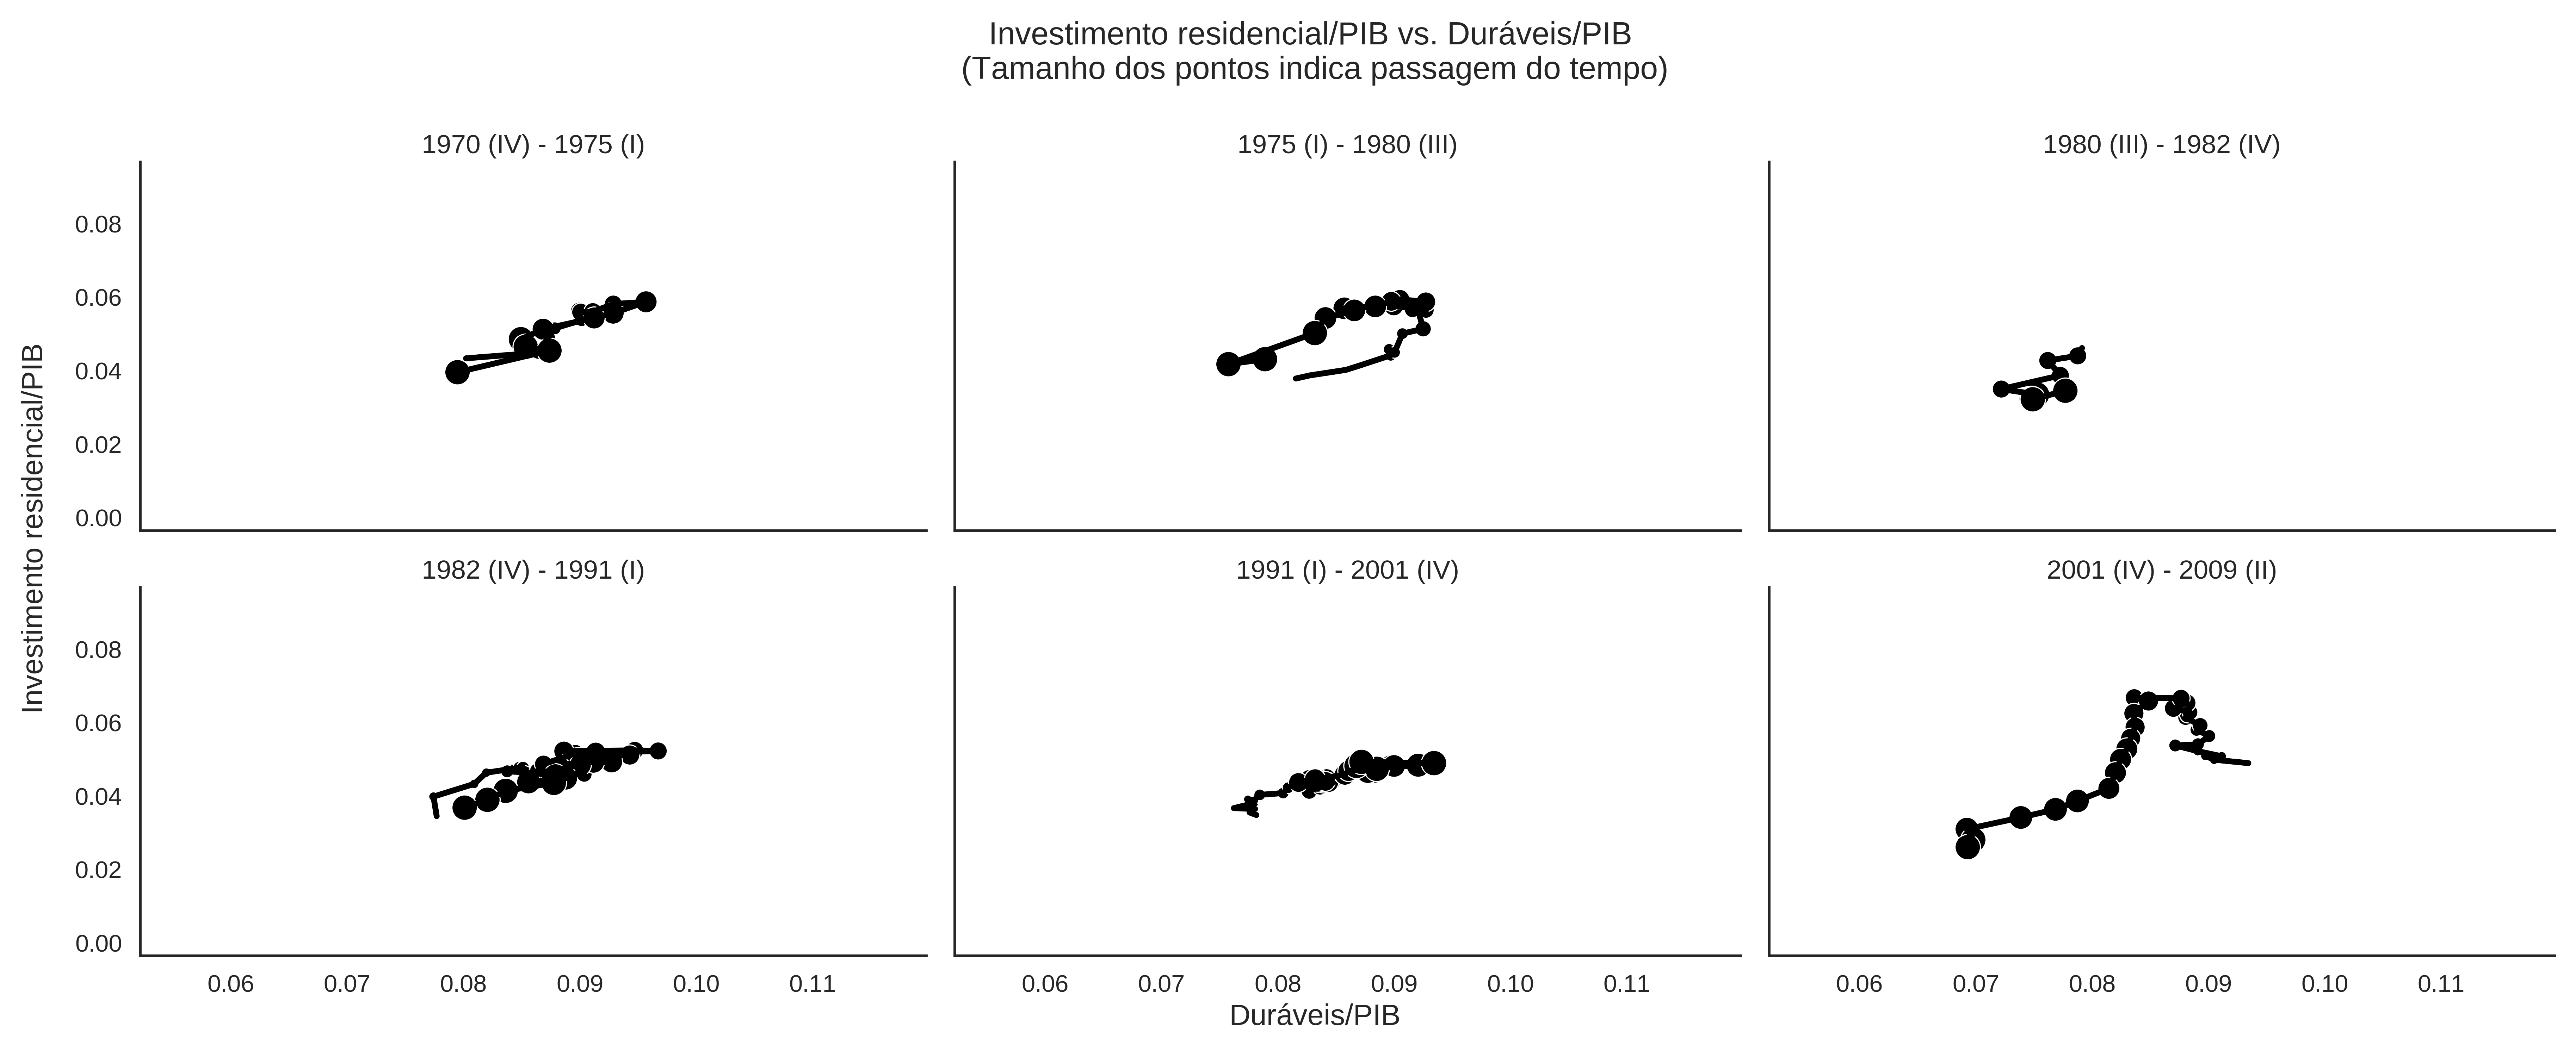
\includegraphics[width=\textwidth]{../../Dados/Fatos_Estilizados/figs/Ciclo_Ih_Duraveis.png}
	\caption*{\textbf{Fonte:} Elaboração própria}
\end{figure}

Desse modo, conclui-se que o investimento residencial ajuda a compreender os ciclos econômicos americanos.
Resta evidenciar como a compreensão deste componente da demanda permite esclarecer tanto as recessões quanto as retomadas. Esta dinâmica poder ser visualizada nos gráficos \ref{FigCriseNorm} e \ref{FigRecuperacaoNorm} em que são apresentadas algumas taxas de crescimento\footnote{Nestes gráficos, as taxas de crescimento são normalizadas para facilitar a comparatibilidade uma vez que é mantida uma mesma escala.} nos trimestres que antecedem e sucedem as recessões/recuperações. 
No que toca as recessões, destaca-se a redução da taxa de crescimento do investimento residencial nos trimestres antecedentes enquanto nas recuperações passa a ter taxas positivas, liderando a recuperação.
Em outras palavras, observa-se que o investimento residencial possui uma taxa de crescimento (a taxas crescentes) positiva nos trimestres que antecedem a recuperação enquanto o investimento das firmas só apresenta tal comportamento adiante. Portanto, esse gráfico ilustra tanto a capacidade do investimento residencial liderar o ciclo quanto a indução do investimento criador de capacidade produtiva.


\begin{figure}[H]
	\centering
	\caption{Taxas de crescimento por recessões antes e depois do início da crise (normalizadas pelo desvio-padrão)}
	\label{FigCriseNorm}
	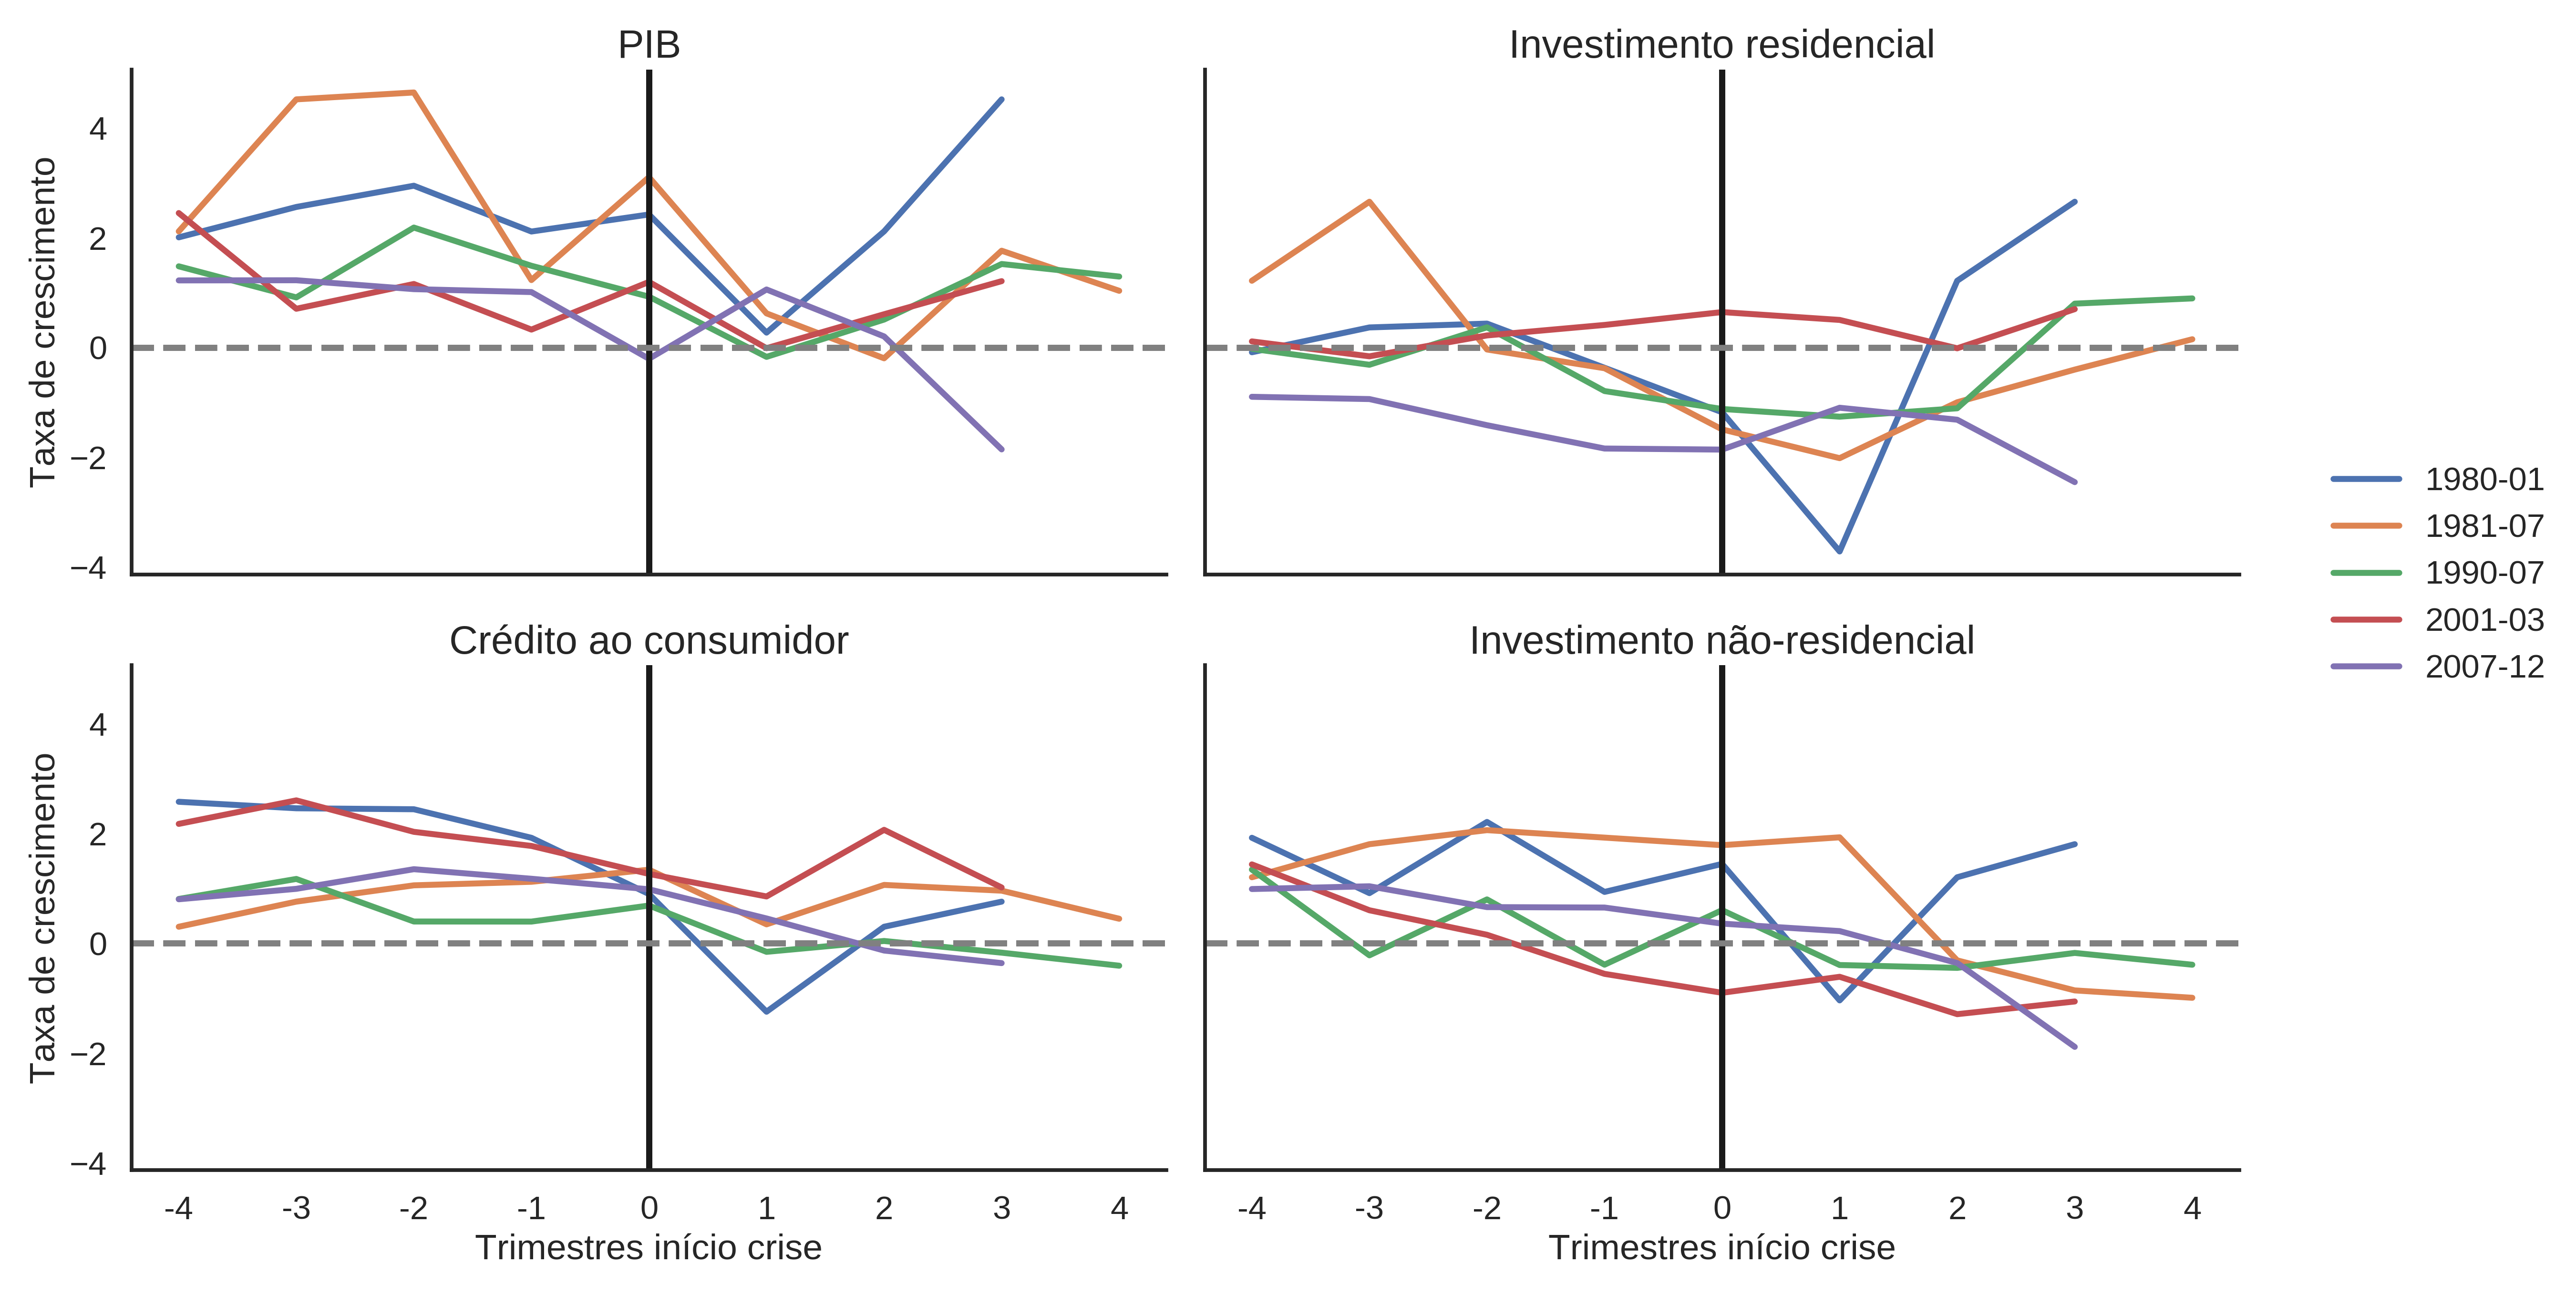
\includegraphics[width=\textwidth]{../../Dados/Fatos_Estilizados/figs/Centrado_Inicio_Norm.png}
	\caption*{\textbf{Fonte:} Elaboração própria}
\end{figure}

\begin{figure}[H]
	\centering
	\caption{Taxas de crescimento por recessões antes e depois do início da recuperação (normalizadas pelo desvio-padrão)}
	\label{FigRecuperacaoNorm}
	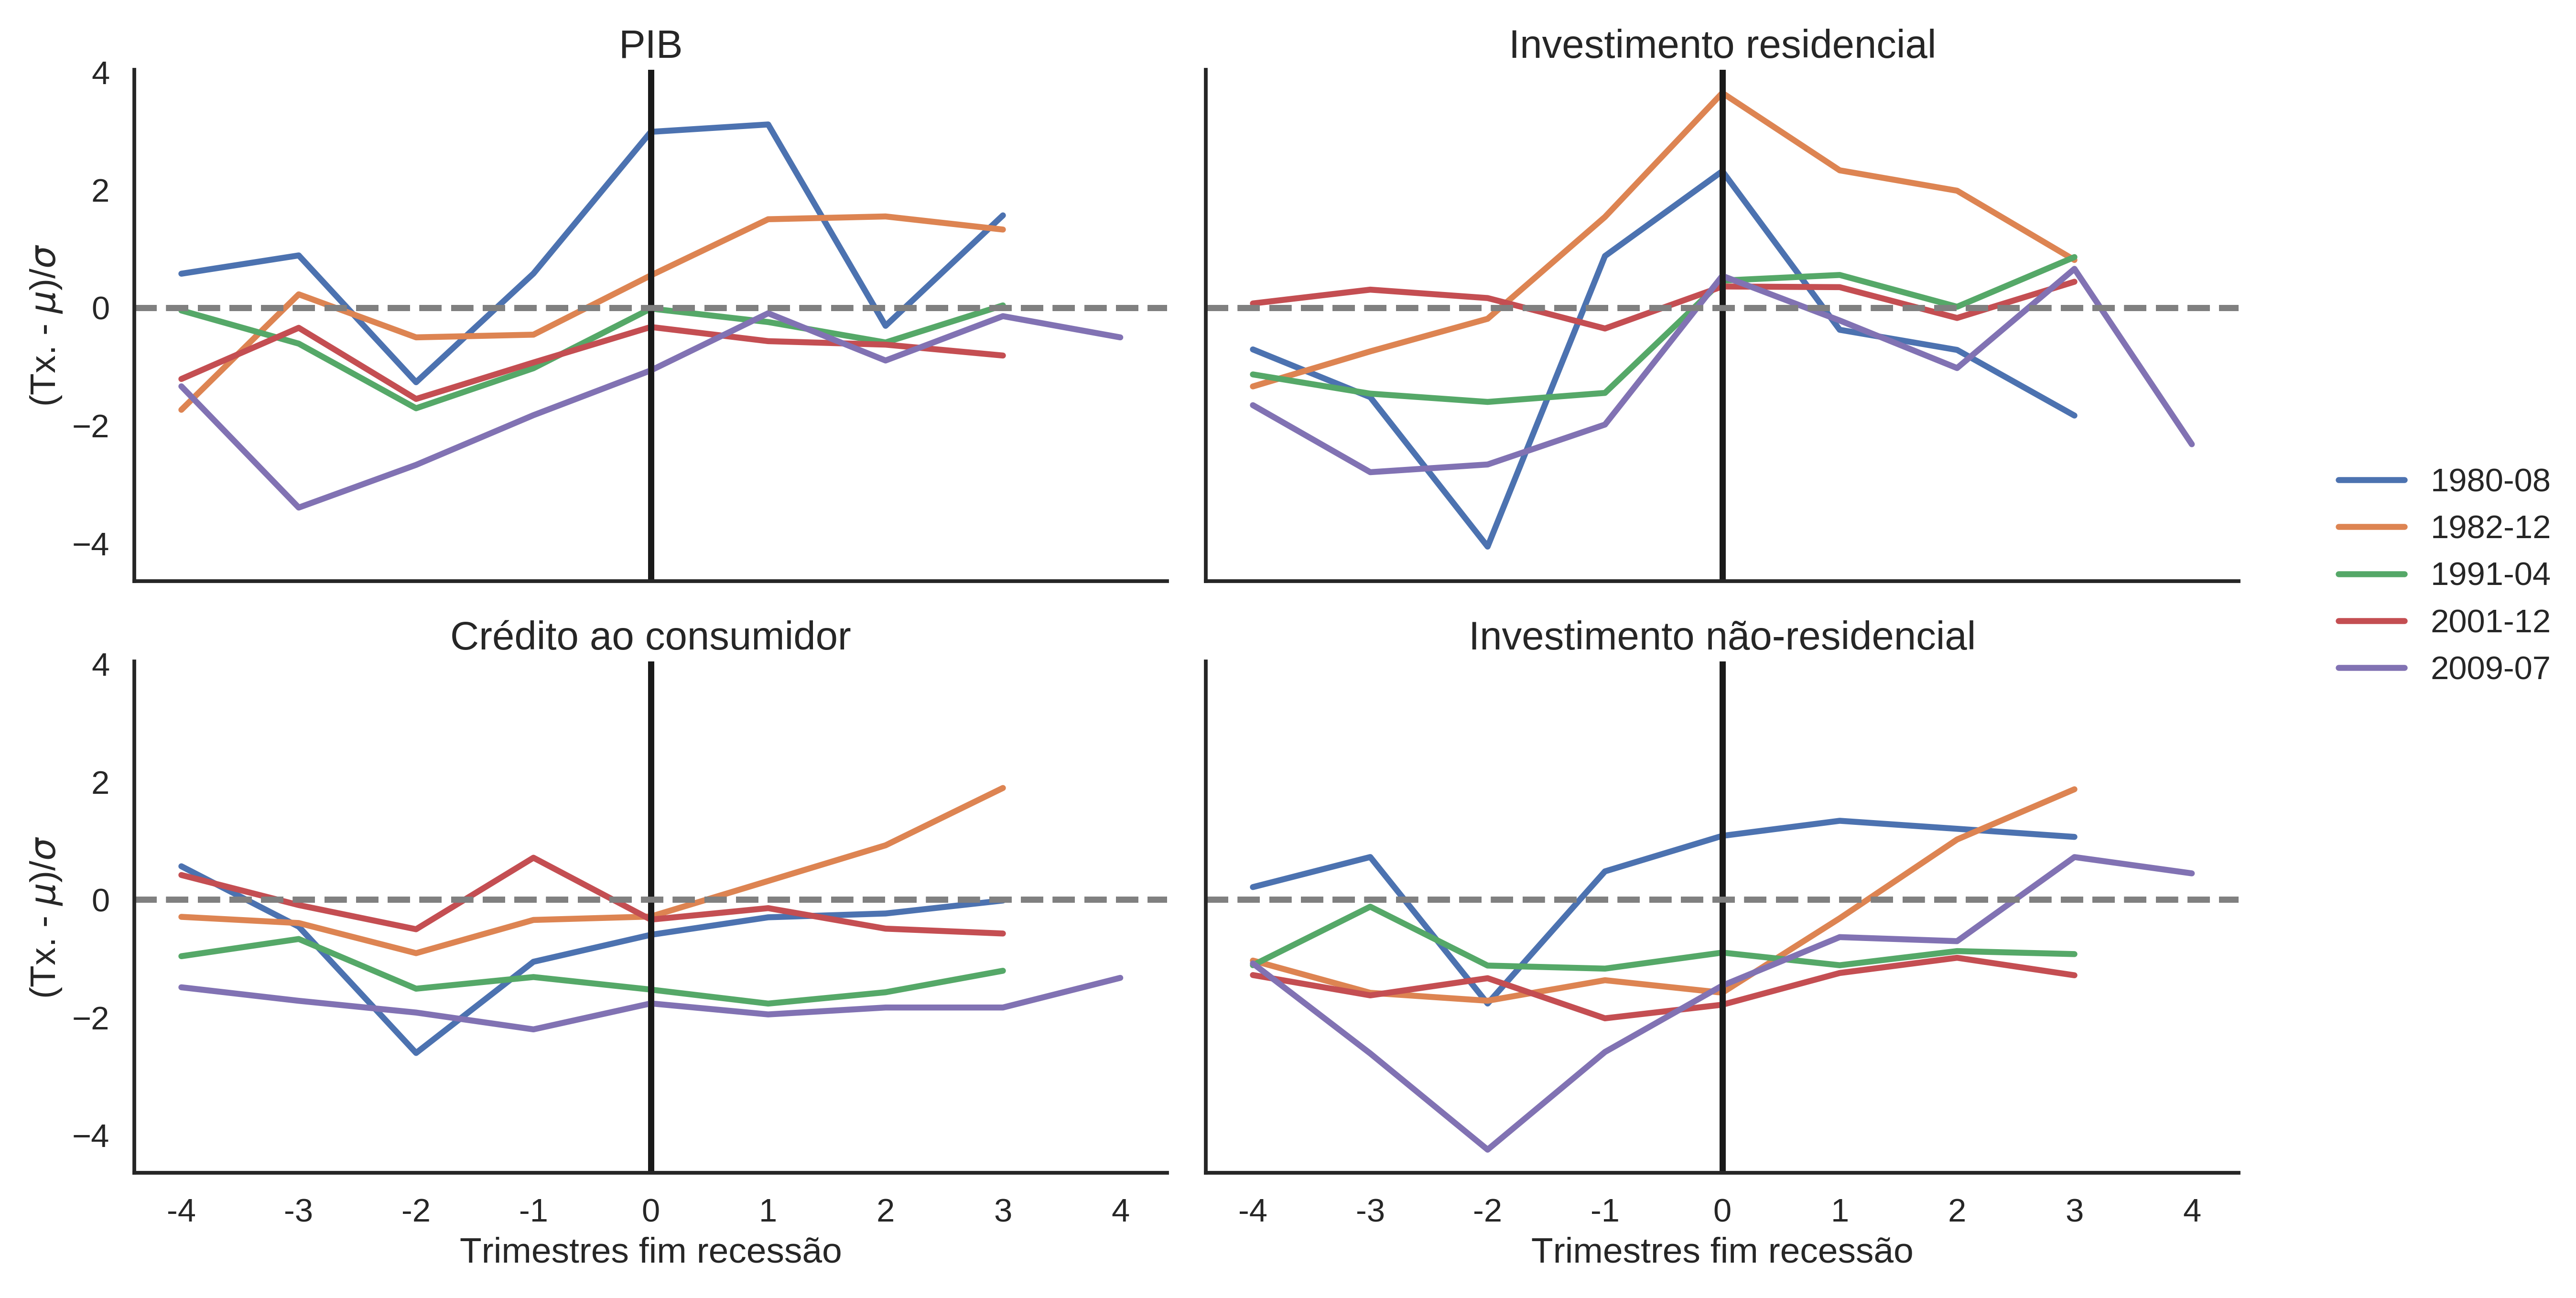
\includegraphics[width=\textwidth]{../../Dados/Fatos_Estilizados/figs/Centrado_Fim_Norm.png}
	\caption*{\textbf{Fonte:} Elaboração própria}
\end{figure}

%TODO Melhorar resolução do gráfico e linhas


Da discussão anterior, conclui-se que a caracterização do ciclo econômico como liderado pelo investimento residencial é bastante extensa uma vez que apresenta esta configuração desde o pós-guerra\footnote{
	A influência deste gasto, no entanto, não se restringe ao crescimento, mas se estende também para questões envolvendo desenvolvimento econômico como visto em um amplo debate iniciado por Duccio A. Turin \cite{pheng_revisit_1992}.}.
No entanto, existêm mudanças significantes --- que não anulam a relevância do investimento residencial --- no pós-década de 80 que precisam ser analisadas em maior detalhe.
Um primeiro elemento é a estagnação salarial e os respectivos efeitos sobre o endividamento das famílias na calda inferior da distribuição \cites{barba_rising_2009}{teixeira_uma_2011}. 
Este endividamento, no entanto, não foi destinado a uma ampliação desproporcional do consumo, mas sim para a preservação do consumo habitual das famílias
\cite{wolf_rising_2010} REFERÊNCIAS.



Estas mudanças distributivas tiveram impactos que vão além efeitos sobre a demanda agregada e se estendem para a recomposição de ativos (reais e financeiros) entre os estratos de renda.
Analisando os ativos (gráfico \ref{FigDistAtivos}), destaca-se que os 50\% mais pobres ganharam participação relativa dos imóveis se comparado com 1979 até meados dos anos 90 ---  comportamento este espelhado pelos 1\% mais ricos. 
Em outras palavras, os imóveis passaram a compor uma parcela cada vez maior do portfólio de ativos deste estrato de renda enquanto os ativos financeiros apresentaram uma tendência de queda persistente.
Enquanto a participação dos imóveis dentre os mais pobres foi oscilante ao longo do período, o mesmo não pode ser dito sobre os bens duráveis, indicando já mencionada tentativa manutenção do padrão de consumo frente a estagnação salarial.


\begin{figure}[H]
	\centering
	\caption{Distribuição de ativos por percentil de riqueza (1979=100)}
	\label{FigDistAtivos}
	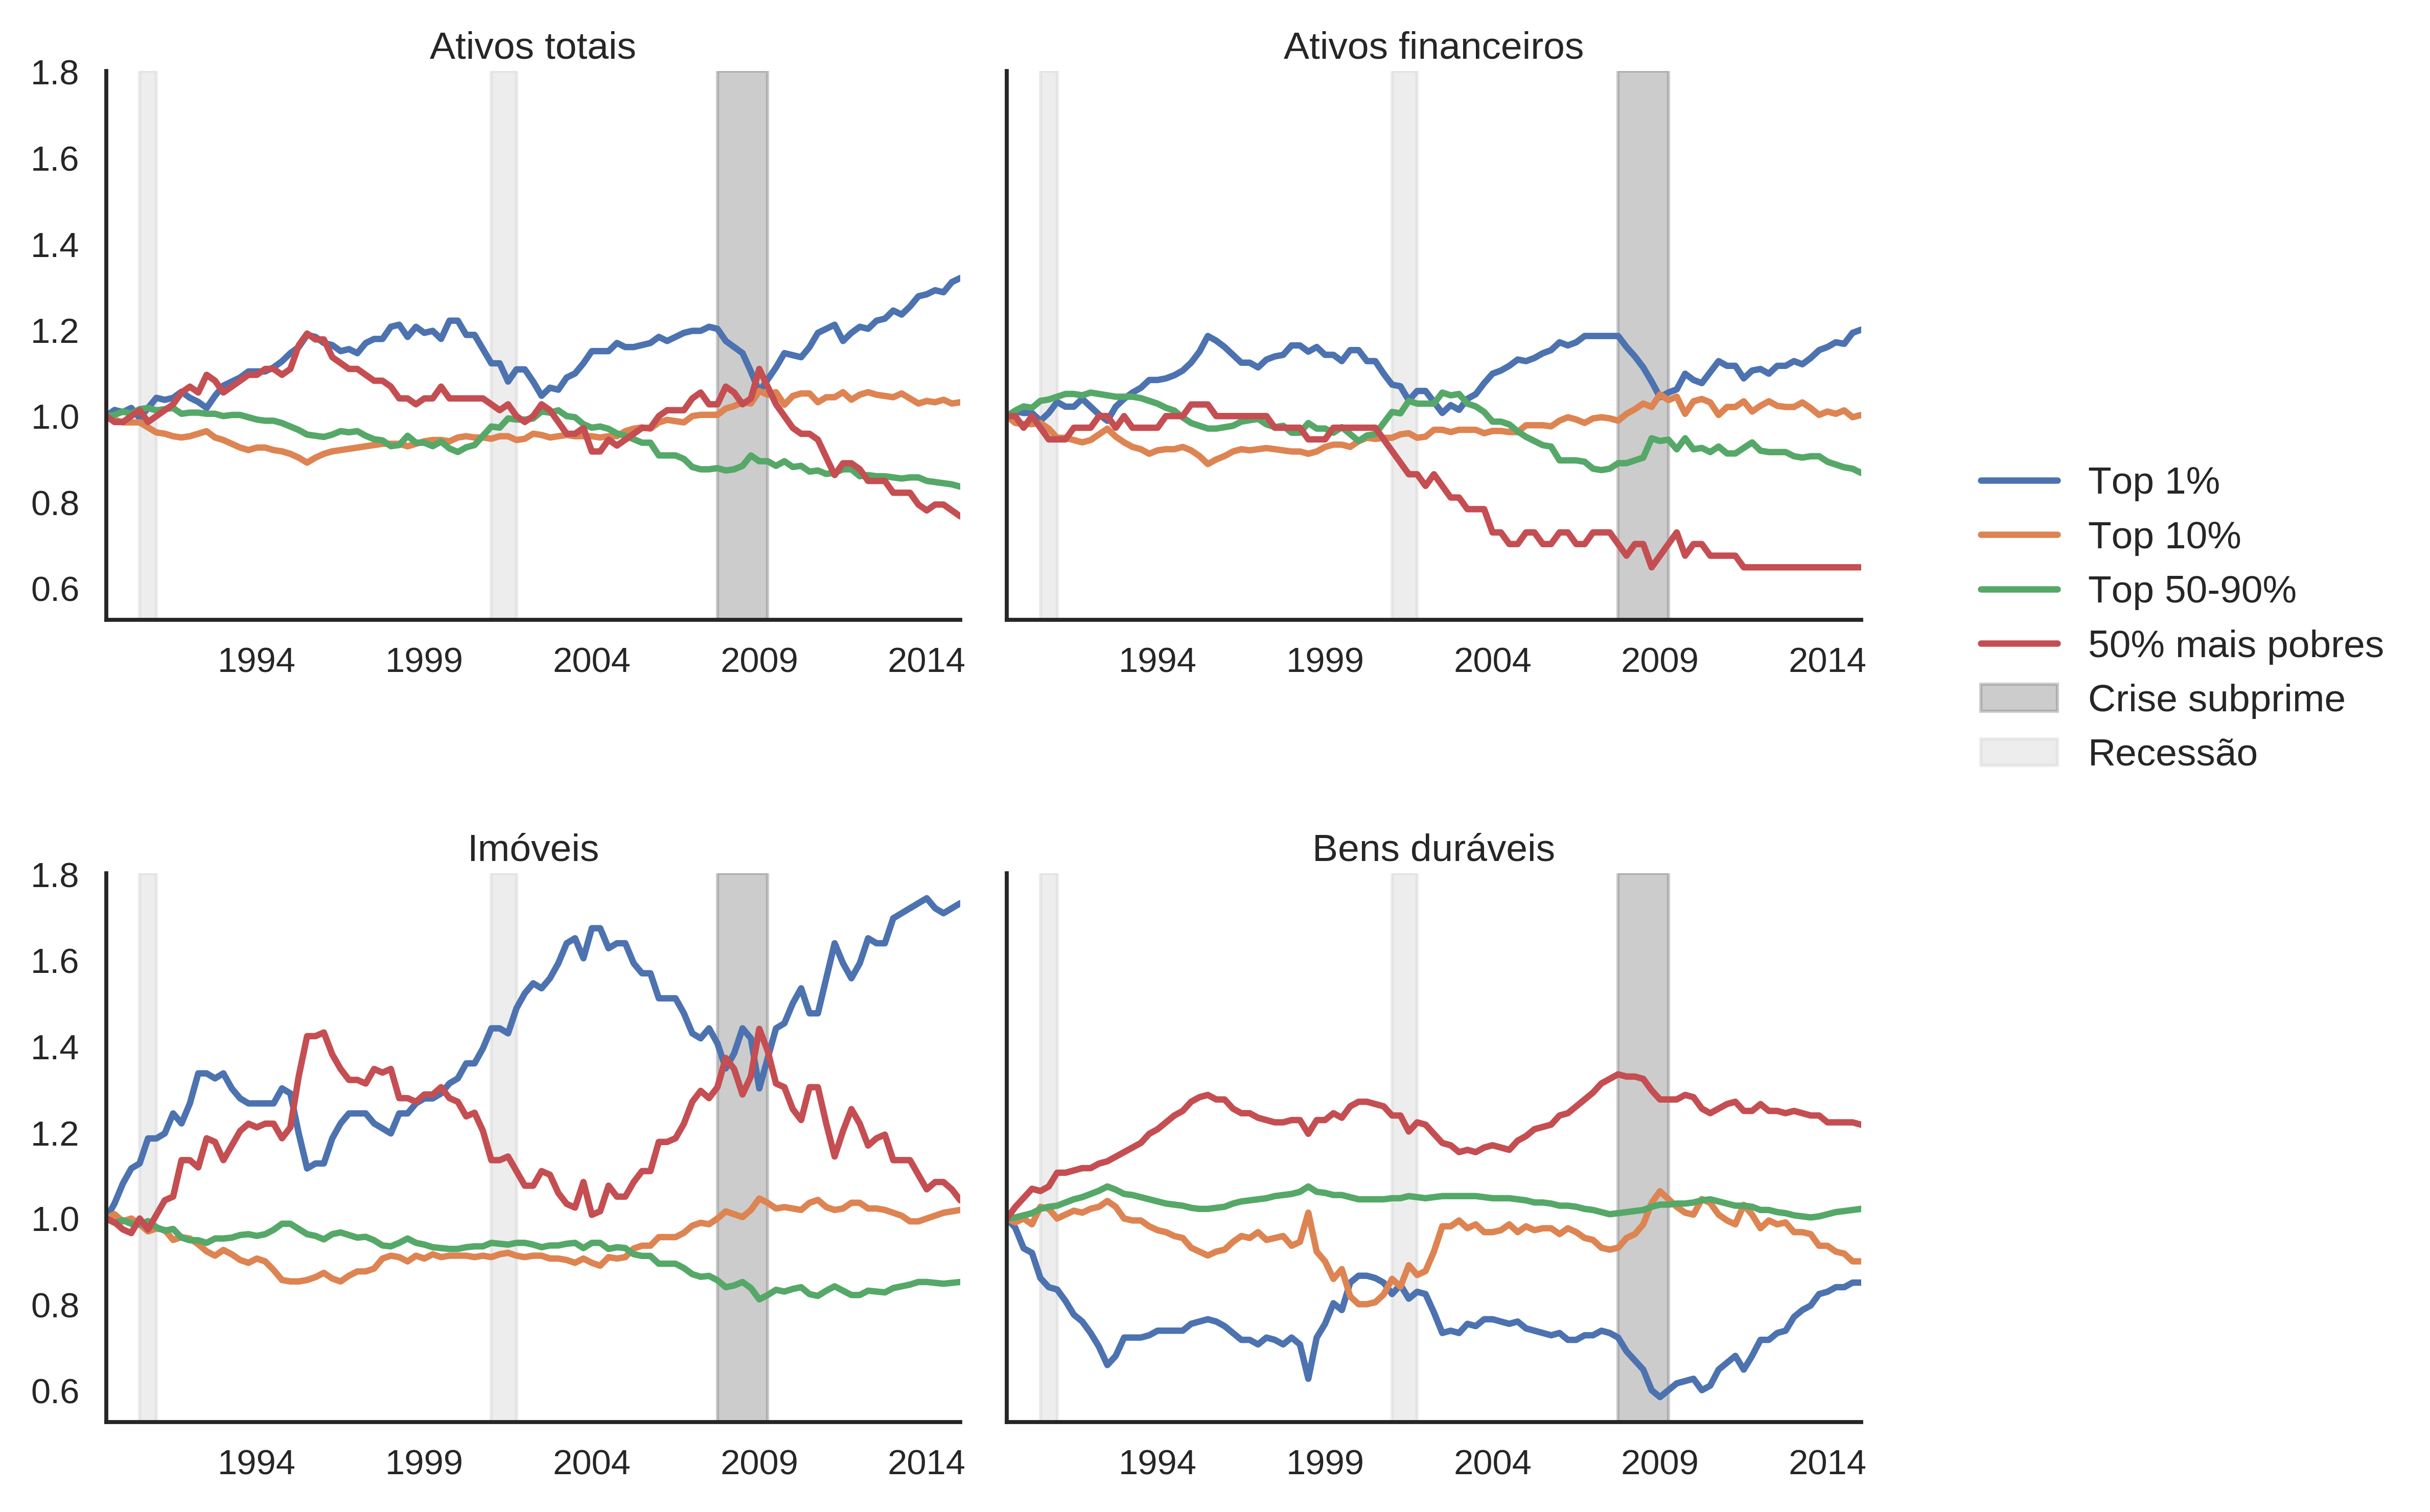
\includegraphics[width=\textwidth]{../../Dados/Fatos_Estilizados/figs/Distribuicao_Ativos.png}
	\caption*{\textbf{Fonte:} \textcite{us_census_bureau_characteristics_2017}, Elaboração própria}
\end{figure}

Os passivos (gráfico \ref{FigDistPassivos}), por sua vez, apresentam uma dinâmica semelhante entre si, ou seja, a participação nos empréstimos e nas hipotecas apresenta é bastante similar ao longo do período analisado e tal resultado decorre da permissividade institucional americana.
De acordo com \textcite{teixeira_uma_2011}, os imóveis são uma das formas de riqueza mais comuns entre as famílias norte-americanas, servindo de colateral para tomada de crédito. A forma de ``realizar'' o ganho de capital com a bolha imobiliária que ocorreu no período, sem precisar liquidar os imóveis, era justamente ampliando o endividamento à medida que o colateral (\textit{i.e.} imóveis) aumentava de valor \cite{teixeira_crescimento_2015}. 


\begin{figure}[H]
	\centering
	\caption{Distribuição de passivos por percentil de riqueza (1979=100)}
	\label{FigDistPassivos}
	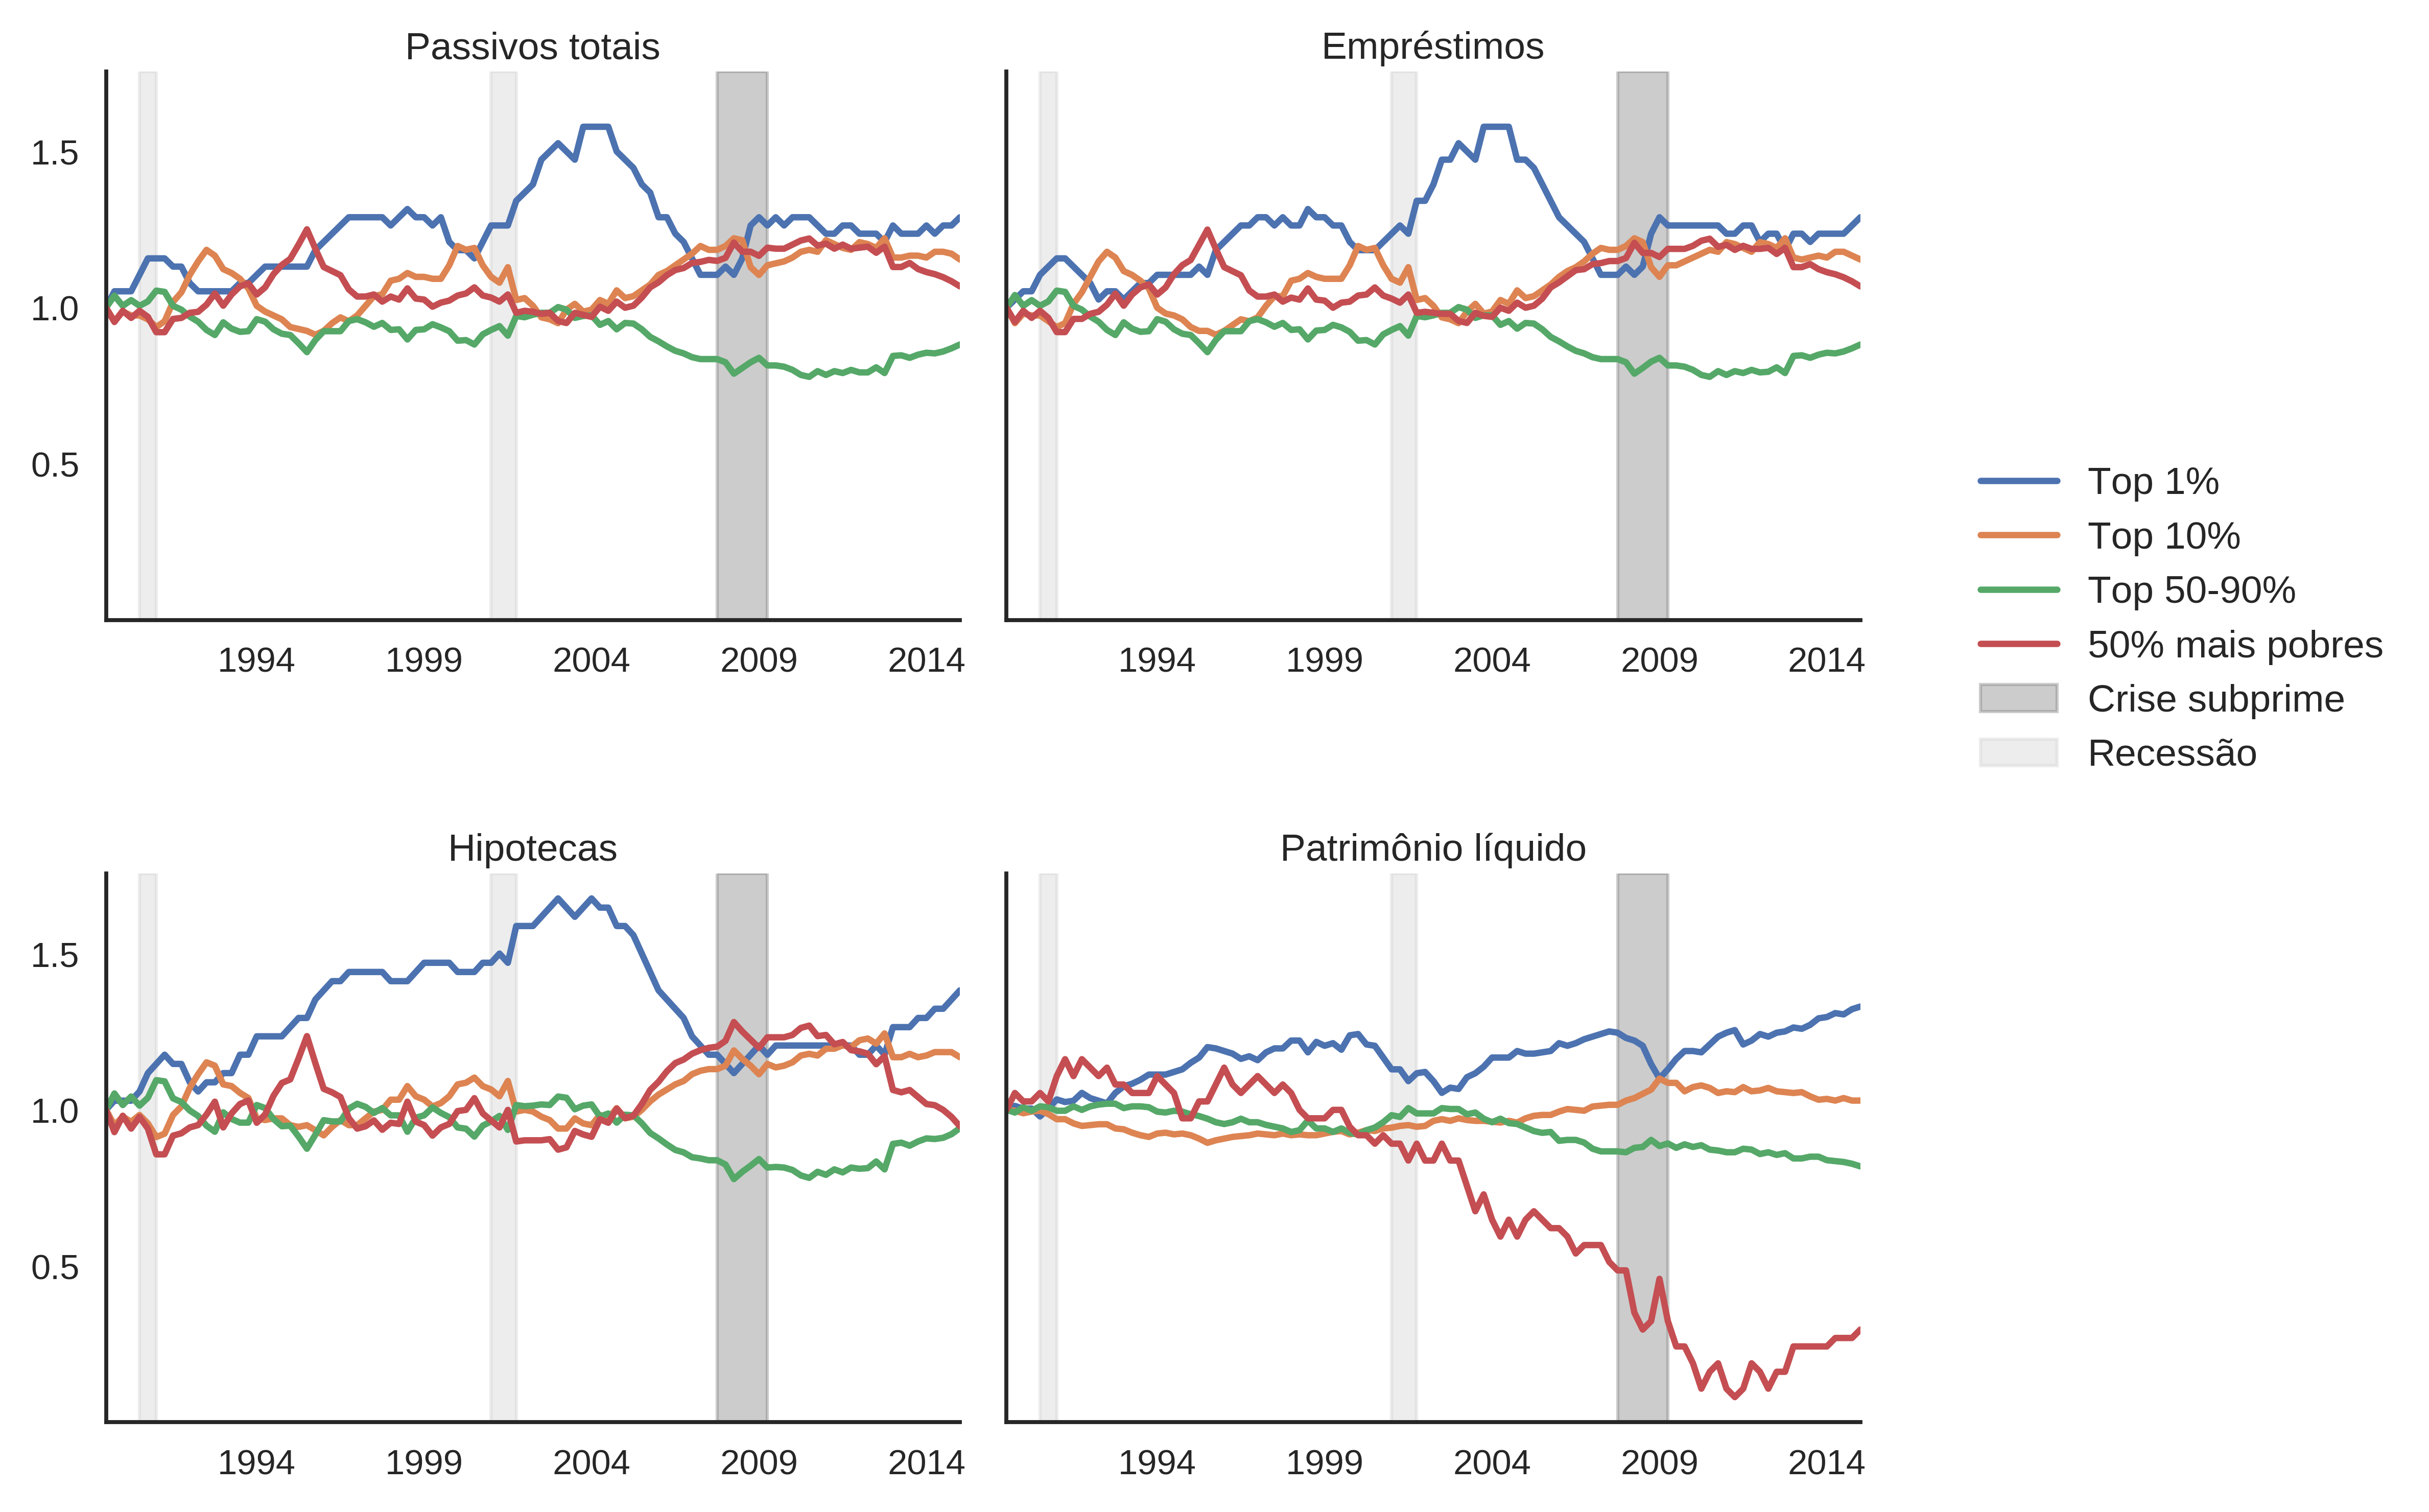
\includegraphics[width=\textwidth]{../../Dados/Fatos_Estilizados/figs/Distribuicao_Passivos.png}
	\caption*{\textbf{Fonte:} \textcite{us_census_bureau_characteristics_2017}, Elaboração própria}
\end{figure}


Desse modo, observa-se uma dinâmica gêmea (ver gráfico \ref{FigDividaPreco}) entre endividamento das famílias e preço dos imóveis que, por sua vez, permitia a ampliação do consumo --- sobretudo das famílias mais pobres --- mesmo com a estagnação salarial do período.
Tal especificidade institucional teve algumas implicações sobre a dinâmica macroeconômica que precisam ser melhor analisadas.
A primeira delas é o descolamento entre ativos e passivos no decorrer da crise financeira de 2008.
Esta separação decorre tanto do esgotamento da bolha dos imóveis que fez com que os tais ativos desvalorizassem quanto da insensibilidade dos compromissos financeiros das famílias (\textit{i.e.} dívida) a queda do preço dos imóveis.
A segunda implicação --- resultante da conjugação dos movimentos anteriores --- é a redução acentuada do patrimônio líquido das famílias mais pobres em termos absolutos ou relativos (painel inferior direito do gráfico \ref{FigDistPassivos}).



\begin{figure}[H]
	\centering
	\caption{Dinâmica do endividamento das famílias e do preço dos imóveis (jan/2000=100)}
	\label{FigDividaPreco}
	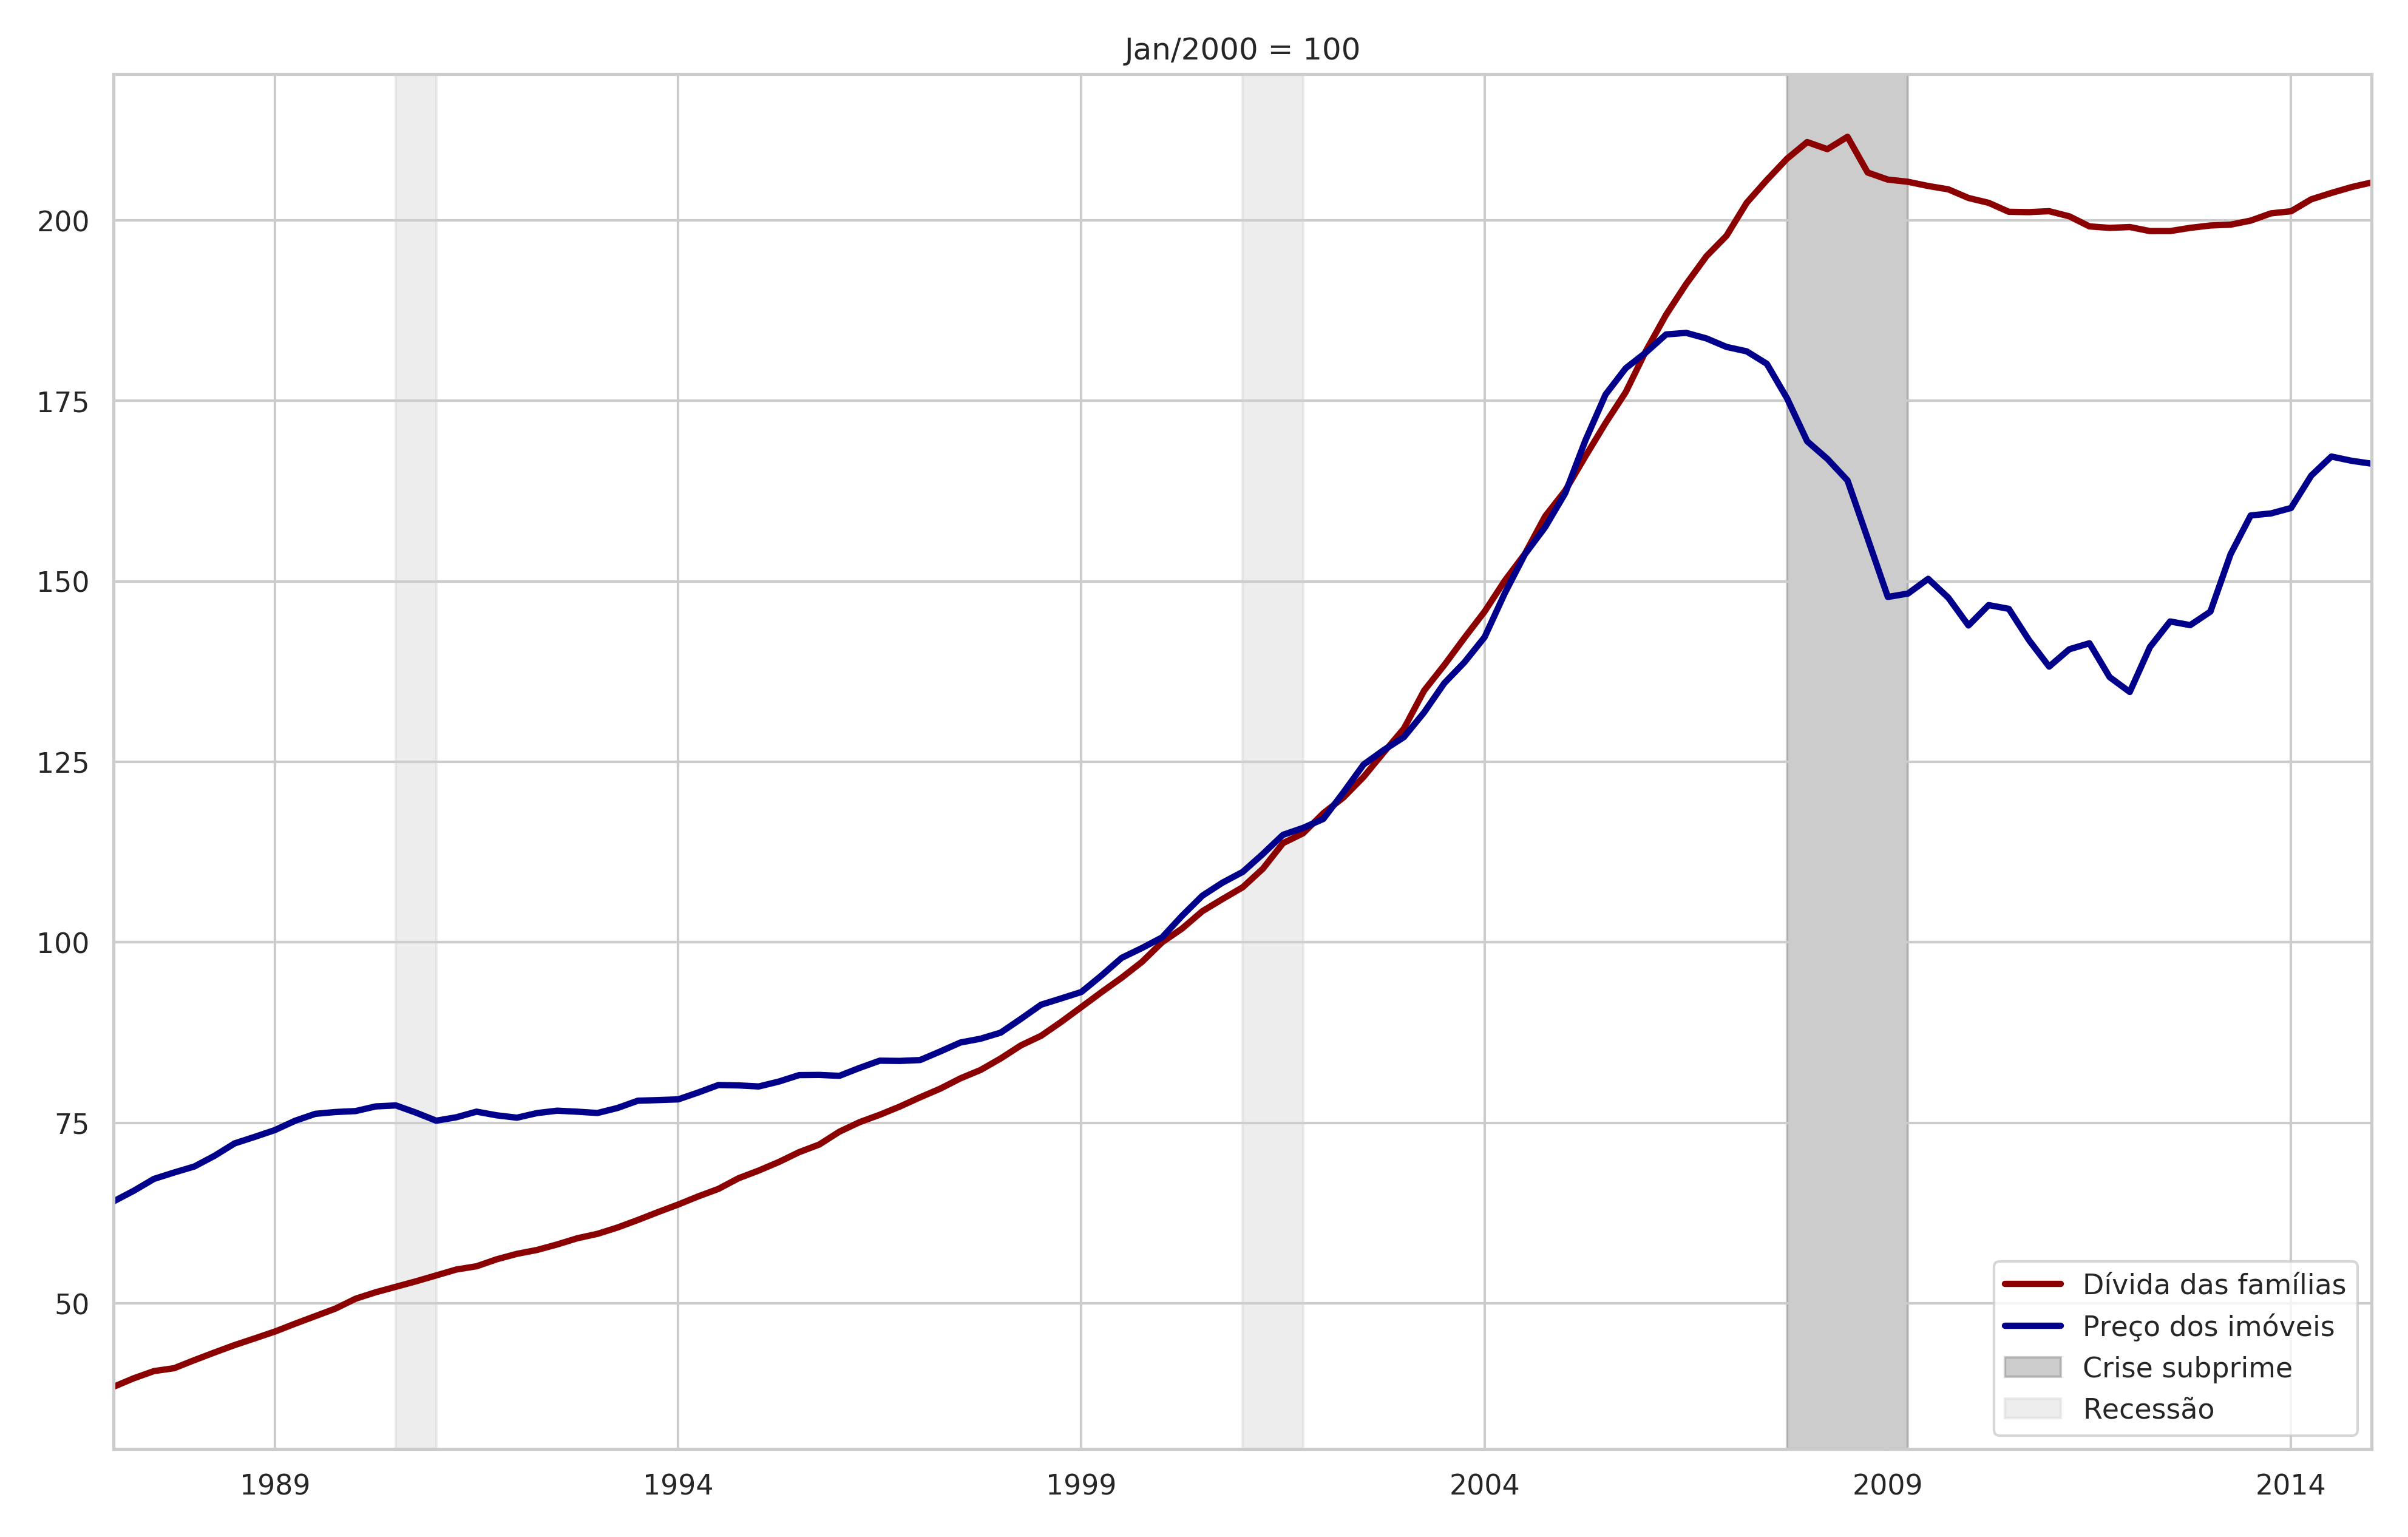
\includegraphics[width=\textwidth]{../../Dados/Fatos_Estilizados/figs/Divida_PrecoImoveis.png}
	\caption*{\textbf{Fonte:} U.S. Bureau of Economic Analisys, elaboração própria}
\end{figure}

REVER

Portanto, a estagnação dos salários somada às inovações financeiras que permitiram ampliação do consumo por meio de ampliação no colateral das famílias associado a elevação do preços dos imóveis.
Esta constatação levou \textcite{barba_rising_2009} a concluirem que tal dinâmica seria sustentável uma vez que houve tanto ampliação do exército de endividados quanto redução das taxas de juros.
No entanto, tais autores desconsideram --- além das inovações financeiras já mencionadas --- um elemento bastante importante: democratização dos imóvies.

A ampliação do acesso a imóveis --- primários, principalmente --- pode ser visualizada no gráfico \ref{FigConcentracao} em que estão apresentadas as curvas de concentração de 1989 a 2010 por diferentes tipos de imóveis.
Em linhas gerais, curvas de concentração são elaboradas a partir da ordenação das famílias --- neste caso, famílias com algum tipo de riqueza --- no eixo horizontal enquanto o eixo vertical apresenta a participação acumulada  pela ordenação de determinado tipo de ativo --- imóveis primários e secundários --- enquanto a reta de 45º indica a linha de perfeita igualdade\footnote{Vale notar que a curva de Lorenz é um tipo específico de curva de concentração em que o eixo vertical apresenta a ordenação acumulada da renda.}.
A partir das curvas de concentração é possível avaliar quão concentrado é certo tipo de ativo em que quão mais acima e a esquerda da linha de perfeita igualdade menos concentrado o ativo em questão está.
Dito isso, uma breve inspeção deste gráfico revela que os anos que antecederam a crise dos \textit{subprime} foram caracterizados pela desconcetração dos imóveis primários, ou seja, estratos mais pobres da riqueza passaram a deter uma parcela acumulada maior deste tipo de imóvel.
O mesmo não pode ser dito sobre os imóveis secundários cujo movimento de concentração/distribuição não é tão demarcado quanto no caso anterior.



%TODO Citar Survey

\begin{figure}[H]
	\centering
	\caption{Curva de concentração por tipos de imóveis}
	\label{FigConcentracao}
	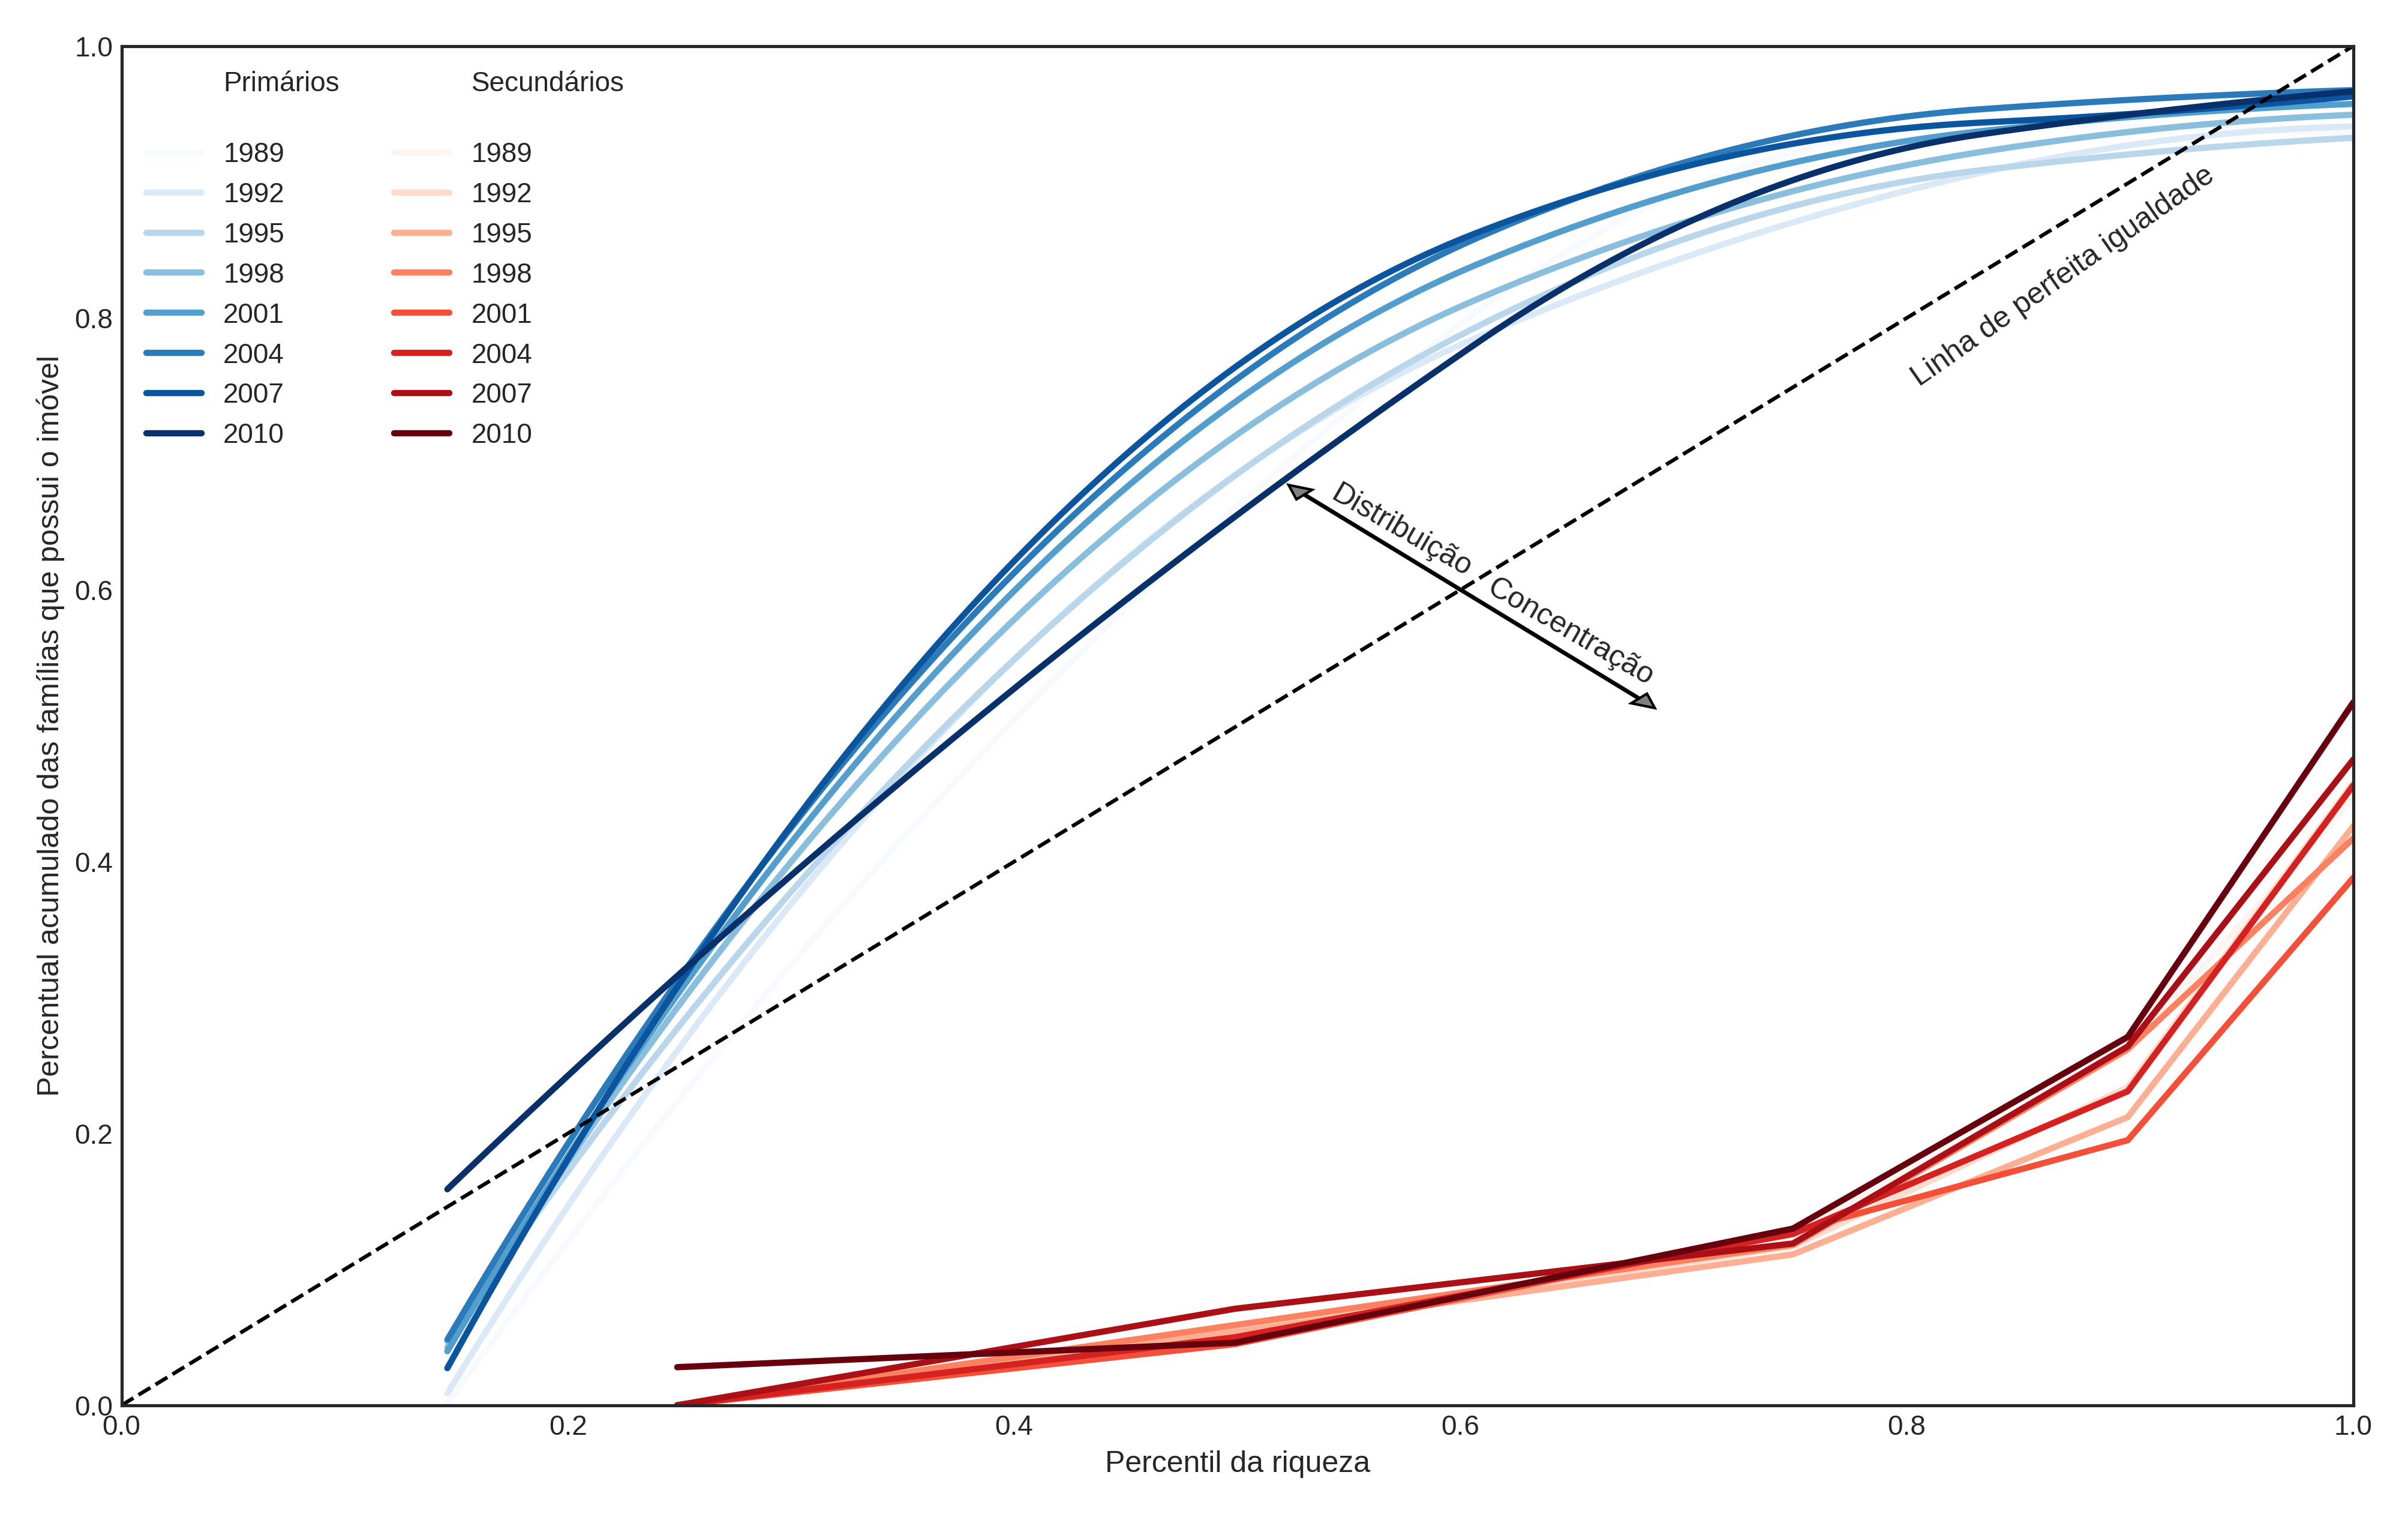
\includegraphics[width=\textwidth]{../../Dados/Fatos_Estilizados/figs/Concentracao_Imoveis.png}
	\caption*{\textbf{Fonte:} \textcite{us_census_bureau_characteristics_2017}, Elaboração própria}
\end{figure}


IMÓVEIS PRIMÁRIOS POR QUE SÃO ÚTEIS E SECUNDÁRIOS PELA ESPECULAÇÃO

A relevância deste movimento é o maior grau de dependência de um número crescente de agentes econômicos da preservação das escalada dos preços dos imóveis.
Sendo assim, uma vez esgotada a bolha de ativos os impactos são maiores que na ausência desta desconcentração de imóveis.
Isso somado a deterioração do patrimônio líquido das famílias mais pobres bem como maior comprometimento da renda disponível com o pagamento de juros contribuiu para o delongamento da retomada da crise recente.

Por fim, cabe pontuar que explicar os determinantes da crise dos \textit{subprime} assim como a inflação de ativos fogem dos objetivos desta pesquisa.
O ponto a ser destacado é a relevância do investimento residencial para dinâmica macroeconômica que não se restringe as mudanças distributivas discutidas acima.


RESUMO PARA OS CHOQUES

%Teixeira e a taxa própria
